%%%%%%%%%%%%%%%%%%%%%%%%%%%%%%%%%%%%%%%%%
% Beamer Presentation
% LaTeX Template
% Version 2.0 (March 8, 2022)
%
% This template originates from:
% https://www.LaTeXTemplates.com
%
% Author:
% Vel (vel@latextemplates.com)
%
% License:
% CC BY-NC-SA 4.0 (https://creativecommons.org/licenses/by-nc-sa/4.0/)
%
%%%%%%%%%%%%%%%%%%%%%%%%%%%%%%%%%%%%%%%%%

%----------------------------------------------------------------------------------------
%	PACKAGES AND OTHER DOCUMENT CONFIGURATIONS
%----------------------------------------------------------------------------------------
\documentclass[
  24pt, % Set the default font size, options include: 8pt, 9pt, 10pt, 11pt, 12pt, 14pt, 17pt, 20pt
  %t, % Uncomment to vertically align all slide content to the top of the slide, rather than the default centered
  aspectratio=169, % Uncomment to set the aspect ratio to a 16:9 ratio which matches the aspect ratio of 1080p and 4K screens and projectors
]{beamer}

\graphicspath{{Images/}{./}} % Specifies where to look for included images (trailing slash required)

\usepackage{booktabs} % Allows the use of \toprule, \midrule and \bottomrule for better rules in tables

%----------------------------------------------------------------------------------------
%	SELECT LAYOUT THEME
%----------------------------------------------------------------------------------------

% Beamer comes with a number of default layout themes which change the colors and layouts of slides. Below is a list of all themes available, uncomment each in turn to see what they look like.

%\usetheme{default}
%\usetheme{AnnArbor}
%\usetheme{Antibes}
%\usetheme{Bergen}
%\usetheme{Berkeley}
%\usetheme{Berlin}
\usetheme{Boadilla} %me gusta
%\usetheme{CambridgeUS}
%\usetheme{Copenhagen}
%\usetheme{Darmstadt}
%\usetheme{Dresden}
%\usetheme{Frankfurt}
%\usetheme{Goettingen} %dos dos
%\usetheme{Hannover} %dos dos
%\usetheme{Ilmenau}
%\usetheme{JuanLesPins}
%\usetheme{Luebeck}
%\usetheme{Madrid}
%\usetheme{Malmoe}
%\usetheme{Marburg}
%\usetheme{Montpellier}
%\usetheme{PaloAlto}
%\usetheme{Pittsburgh}
%\usetheme{Rochester} %muy flat
%\usetheme{Singapore}
%\usetheme{Szeged}
%\usetheme{Warsaw}

%----------------------------------------------------------------------------------------
%	SELECT COLOR THEME
%----------------------------------------------------------------------------------------

% Beamer comes with a number of color themes that can be applied to any layout theme to change its colors. Uncomment each of these in turn to see how they change the colors of your selected layout theme.

%\usecolortheme{albatross}
%\usecolortheme{beaver}
%\usecolortheme{beetle}
%\usecolortheme{crane}
%\usecolortheme{dolphin}
%\usecolortheme{dove}
%\usecolortheme{fly}
%\usecolortheme{lily} %default
%\usecolortheme{monarca}
%\usecolortheme{seagull}
%\usecolortheme{seahorse}
%\usecolortheme{spruce}
%\usecolortheme{whale}
%\usecolortheme{wolverine}

%----------------------------------------------------------------------------------------
%	SELECT FONT THEME & FONTS
%----------------------------------------------------------------------------------------

% Beamer comes with several font themes to easily change the fonts used in various parts of the presentation. Review the comments beside each one to decide if you would like to use it. Note that additional options can be specified for several of these font themes, consult the beamer documentation for more information.

\usefonttheme{default} % Typeset using the default sans serif font
%\usefonttheme{serif} % Typeset using the default serif font (make sure a sans font isn't being set as the default font if you use this option!)
%\usefonttheme{structurebold} % Typeset important structure text (titles, headlines, footlines, sidebar, etc) in bold
%\usefonttheme{structureitalicserif} % Typeset important structure text (titles, headlines, footlines, sidebar, etc) in italic serif
%\usefonttheme{structuresmallcapsserif} % Typeset important structure text (titles, headlines, footlines, sidebar, etc) in small caps serif

%------------------------------------------------

%\usepackage{mathptmx} % Use the Times font for serif text
\usepackage{palatino} % Use the Palatino font for serif text

\usepackage[ruled,vlined]{algorithm2e}
%\usepackage{helvet} % Use the Helvetica font for sans serif text
\usepackage[default]{opensans} % Use the Open Sans font for sans serif text
\usepackage[spanish]{babel}
\usepackage{dirtree}
\usepackage{xcolor}
%\usepackage[default]{FiraSans} % Use the Fira Sans font for sans serif text
%\usepackage[default]{lato} % Use the Lato font for sans serif text

\usepackage[scaled]{helvet}
\usepackage[round]{natbib}
%\newcommand{\newblock}{}

\usepackage{rotating}

\newcommand\FourQuad[4]{%
  \begin{minipage}[b][.33\textheight][t] 
    {.48\textwidth}#1\end{minipage}\hfill%
    \begin{minipage}[b][.33\textheight][t] 
      {.48\textwidth}#2\end{minipage}\\[0.5em]
      \begin{minipage}[b][.33\textheight][t] 
        {.48\textwidth}#3\end{minipage}\hfill
        \begin{minipage}[b][.33\textheight][t] 
          {.48\textwidth}#4\end{minipage}%
}

\usepackage{tikz}
%\usetikzlibrary{arrows,shapes,positioning,shadows,trees,quotes}


%\tikzset{
%  basic/.style  = {draw, text width=2cm, drop shadow, font=\sffamily, rectangle},
%  root/.style   = {basic, rounded corners=2pt, thin, align=center,
%                   fill=green!30},
%  level 2/.style = {basic, rounded corners=6pt, thin,align=center, fill=green!60,
%                   text width=8em},
%  level 3/.style = {basic, thin, align=left, fill=pink!60, text width=6.5em}
%}

\usetikzlibrary{calc}

\tikzstyle{part} = [rectangle, rounded corners, minimum width=3cm, minimum height=1cm,     align=center, draw=black]
\tikzstyle{chapter} = [rectangle, rounded corners, minimum width=3cm, minimum height=1cm,     align=center, draw=black, text width=3.5cm]
\tikzstyle{arrow} = [thick, ->]

\usepackage{array} % needed for \arraybackslash
\usepackage{graphicx}
\usepackage{adjustbox} % for \adjincludegraphics

\usepackage{subcaption}
\usepackage{bibentry}
%\bibliographystyle{apalike}
\usepackage{chngcntr}
\usepackage{lipsum}% http://ctan.org/pkg/lipsum
\usepackage{hanging}% http://ctan.org/pkg/hanging

\usepackage{xcolor,colortbl}
\usepackage{multirow}

\usepackage{animate}
\usepackage{multicol}
\usepackage{tabularx,booktabs}
\usepackage{forloop}
\usepackage{ragged2e}

\usepackage{bbding} %palomitas checkmark
\usepackage{pifont}
\usepackage{lipsum,tabularx}
\newcounter{loopcntr}
%----------------------------------------------------------------------------------------
%	SELECT INNER THEME
%----------------------------------------------------------------------------------------

% Inner themes change the styling of internal slide elements, for example: bullet points, blocks, bibliography entries, title pages, theorems, etc. Uncomment each theme in turn to see what changes it makes to your presentation.

%\useinnertheme{default}
\useinnertheme{circles}
%\useinnertheme{rectangles}
%\useinnertheme{rounded}
%\useinnertheme{inmargin}

%----------------------------------------------------------------------------------------
%	SELECT OUTER THEME
%----------------------------------------------------------------------------------------

% Outer themes change the overall layout of slides, such as: header and footer lines, sidebars and slide titles. Uncomment each theme in turn to see what changes it makes to your presentation.

%\useoutertheme{default}
%\useoutertheme{infolines}
%\useoutertheme{miniframes}
%\useoutertheme{smoothbars}
%\useoutertheme{sidebar}
%\useoutertheme{split}
%\useoutertheme{shadow}
%\useoutertheme{tree}
%\useoutertheme{smoothtree}

%\setbeamertemplate{footline} % Uncomment this line to remove the footer line in all slides
\setbeamertemplate{footline}[page number] % Uncomment this line to replace the footer line in all slides with a simple slide count
%\setbeamertemplate{caption}[numbered]
\setbeamertemplate{navigation symbols}{} % Uncomment this line to remove the navigation symbols from the bottom of all slides

%----------------------------------------------------------------------------------------
%	PRESENTATION INFORMATION
%----------------------------------------------------------------------------------------

\title[PROTOCOLO DE INVESTIGACIÓN]{%\centering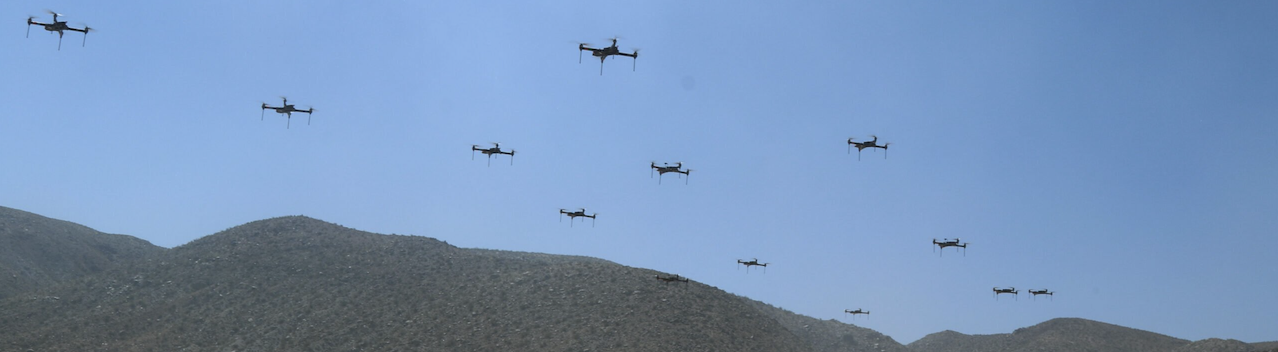
\includegraphics[width=10cm]{swarm_drones}\\
  Estrategias para la exploración coordinada multi-VANT} % The short title in the optional parameter appears at the bottom of every slide, the full title in the main parameter is only on the title page

%\subtitle{Optional Subtitle} % Presentation subtitle, remove this command if a subtitle isn't required

\author[Luis Ballado]{Luis Alberto Ballado Aradias} % Presenter name(s), the optional parameter can contain a shortened version to appear on the bottom of every slide, while the main parameter will appear on the title slide

\institute[CINVESTAV]{
  CINVESTAV UNIDAD TAMAULIPAS \\
  %\smallskip \textit{luis.ballado@cinvestav.mx}
} % Your institution, the optional parameter can be used for the institution shorthand and will appear on the bottom of every slide after author names, while the required parameter is used on the title slide and can include your email address or additional information on separate lines

\date[\today]{Cd. Victoria, Tamaulipas - \today} % Presentation date or conference/meeting name, the optional parameter can contain a shortened version to appear on the bottom of every slide, while the required parameter value is output to the title slide

%\titlegraphic{\hspace*{8.75cm}~%
%   
\includegraphics[width=0.8cm]{cinvestavlogo}
%}

%----------------------------------------------------------------------------------------

\counterwithin*{footnote}{page}
\newcommand\footcite[1]{\footnote{\bibentry{#1}}\label{\thepage:#1}}
\newcommand\secondcite[1]{\textsuperscript{\ref{\thepage:#1}}}

\newcommand{\rpt}[2][1]{%
  \forloop{loopcntr}{0}{\value{loopcntr}<#1}{#2}%
}
\newcommand{\on}[1][1]{
  \forloop{loopcntr}{0}{\value{loopcntr}<#1}{&\cellcolor{gray}}
}
\newcommand{\off}[1][1]{
  \forloop{loopcntr}{0}{\value{loopcntr}<#1}{&}
}

\addtolength{\textheight}{90pt}

\newcommand{\I}{\mathbb{I}}
\newcommand{\K}{\mathbb{K}}
\newcommand{\N}{\mathbb{N}}
\newcommand{\Q}{\mathbb{Q}}
\newcommand{\R}{\mathbb{R}}
\newcommand{\Z}{\mathbb{Z}}

\newcommand{\specialcell}[2][c]{%
  \begin{tabular}[#1]{@{}c@{}}#2\end{tabular}}


\begin{document}

%----------------------------------------------------------------------------------------
%	TITLE SLIDE
%----------------------------------------------------------------------------------------

\begin{frame}
  \titlepage % Output the title slide, automatically created using the text entered in the PRESENTATION INFORMATION block above
\end{frame}

%----------------------------------------------------------------------------------------
%	TABLE OF CONTENTS SLIDE
%----------------------------------------------------------------------------------------

% The table of contents outputs the sections and subsections that appear in your presentation, specified with the standard \section and \subsection commands. You may either display all sections and subsections on one slide with \tableofcontents, or display each section at a time on subsequent slides with \tableofcontents[pausesections]. The latter is useful if you want to step through each section and mention what you will discuss.
\AtBeginSection[]
{
  \begin{frame}
    \frametitle{Contenido} % Slide title, remove this command for no title
    \tableofcontents[currentsection] % Output the table of contents (all sections on one slide)
    %\tableofcontents[pausesections] % Output the table of contents (break sections up across separate slides)
  \end{frame}
}
%----------------------------------------------------------------------------------------
%	PRESENTATION BODY SLIDES
%----------------------------------------------------------------------------------------

\section{Descripción del proyecto}
\begin{frame}{Descripción del proyecto}
  \bigskip % Vertical whitespace
  \centering
  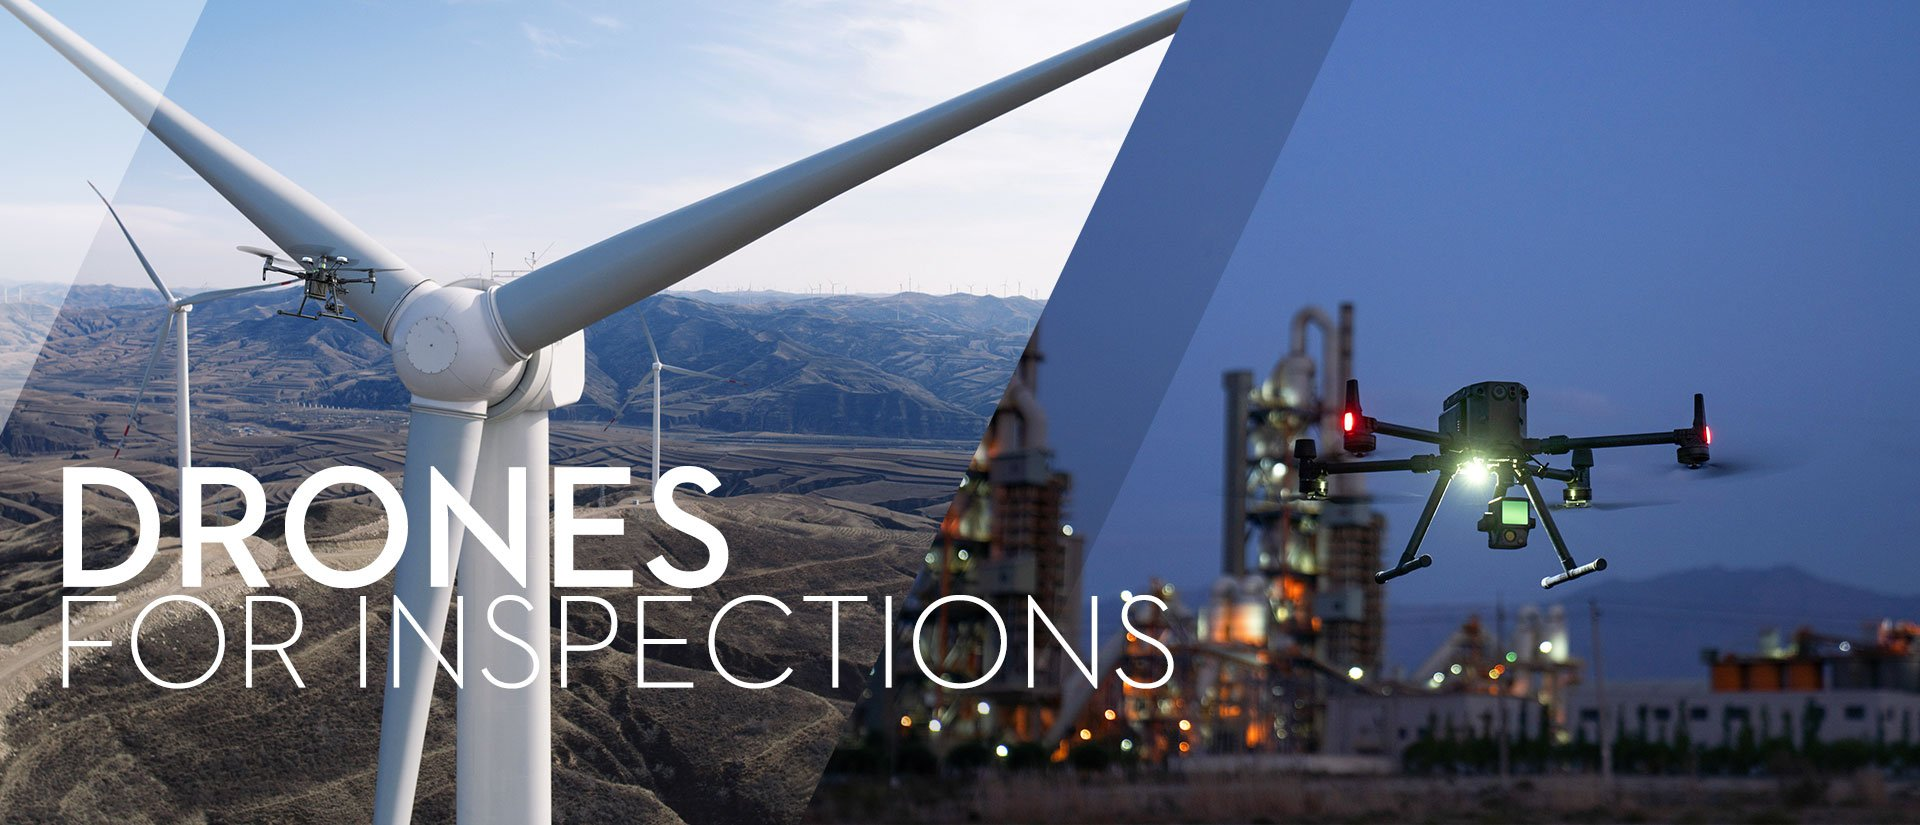
\includegraphics[width=0.45\textwidth,height=0.35\textheight]{DJI_B1}$^\dag$
  \hfil
  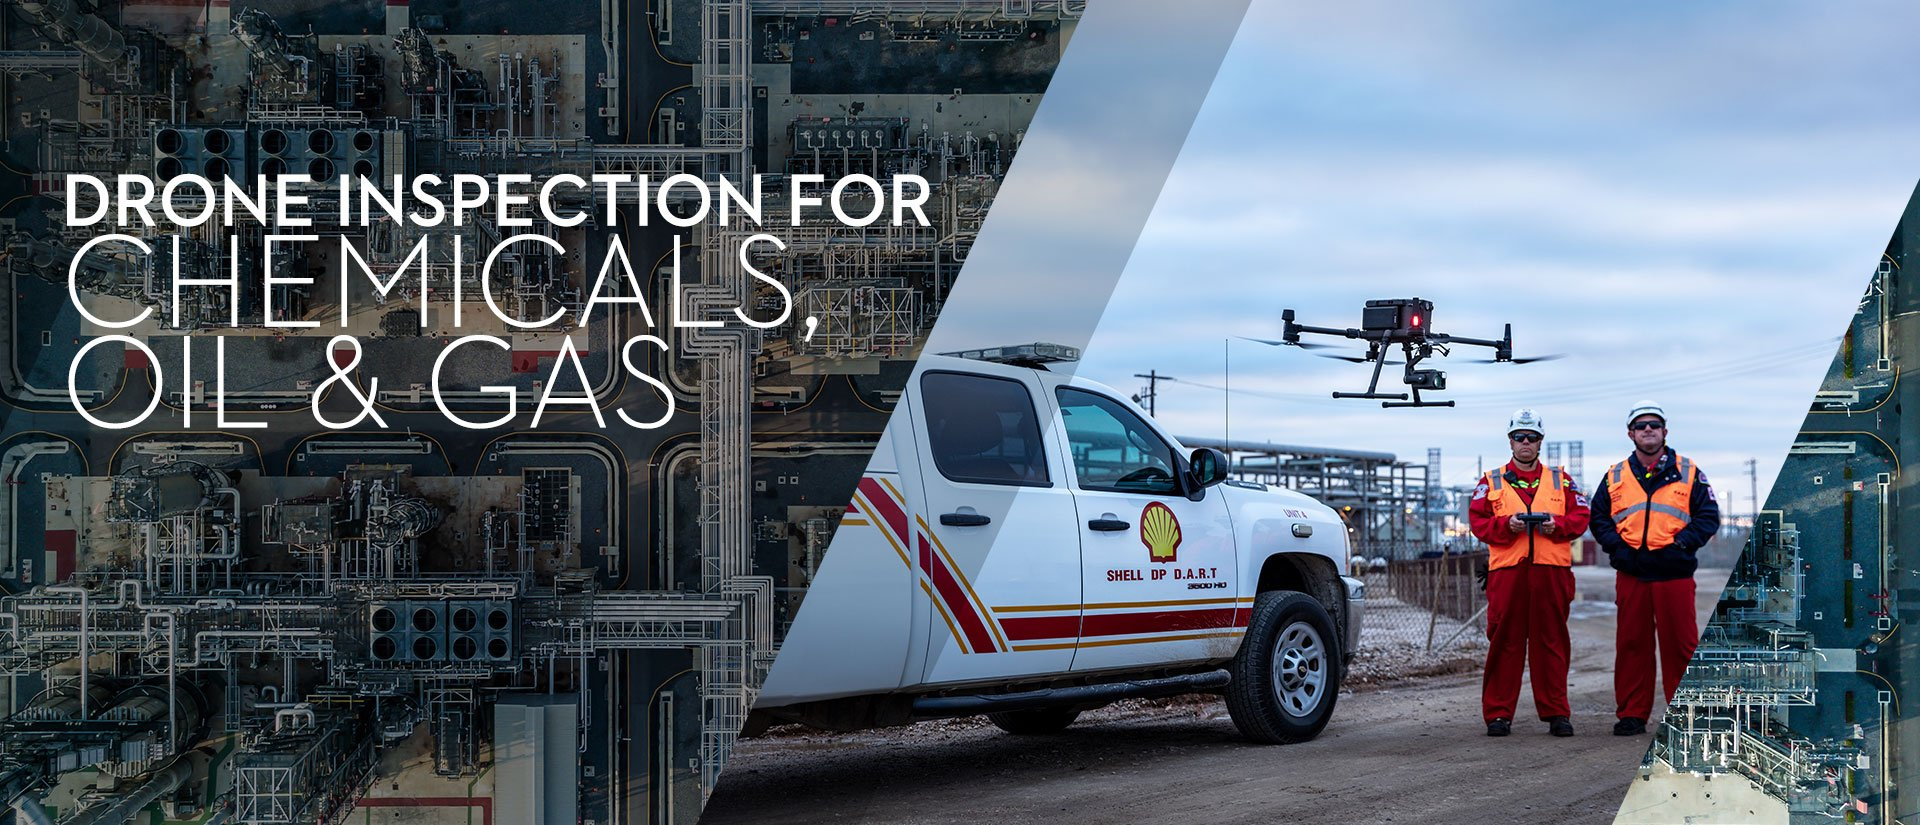
\includegraphics[width=0.45\textwidth,height=0.35\textheight]{DJI_B4}$^\dag$
  \vspace{2pt}\\
  
  \begin{itemize}
  \item \textbf{Aplicaciones} en lugares inaccesibles o peligrosos.
  \item \textbf{Múltiples VANT} pueden reducir el tiempo de exploración y aumentar la confianza del sistema.
  \item \textbf{Limitaciones} en carga, procesamiento y batería influyen en el tiempo de vuelo.
  \end{itemize}

  %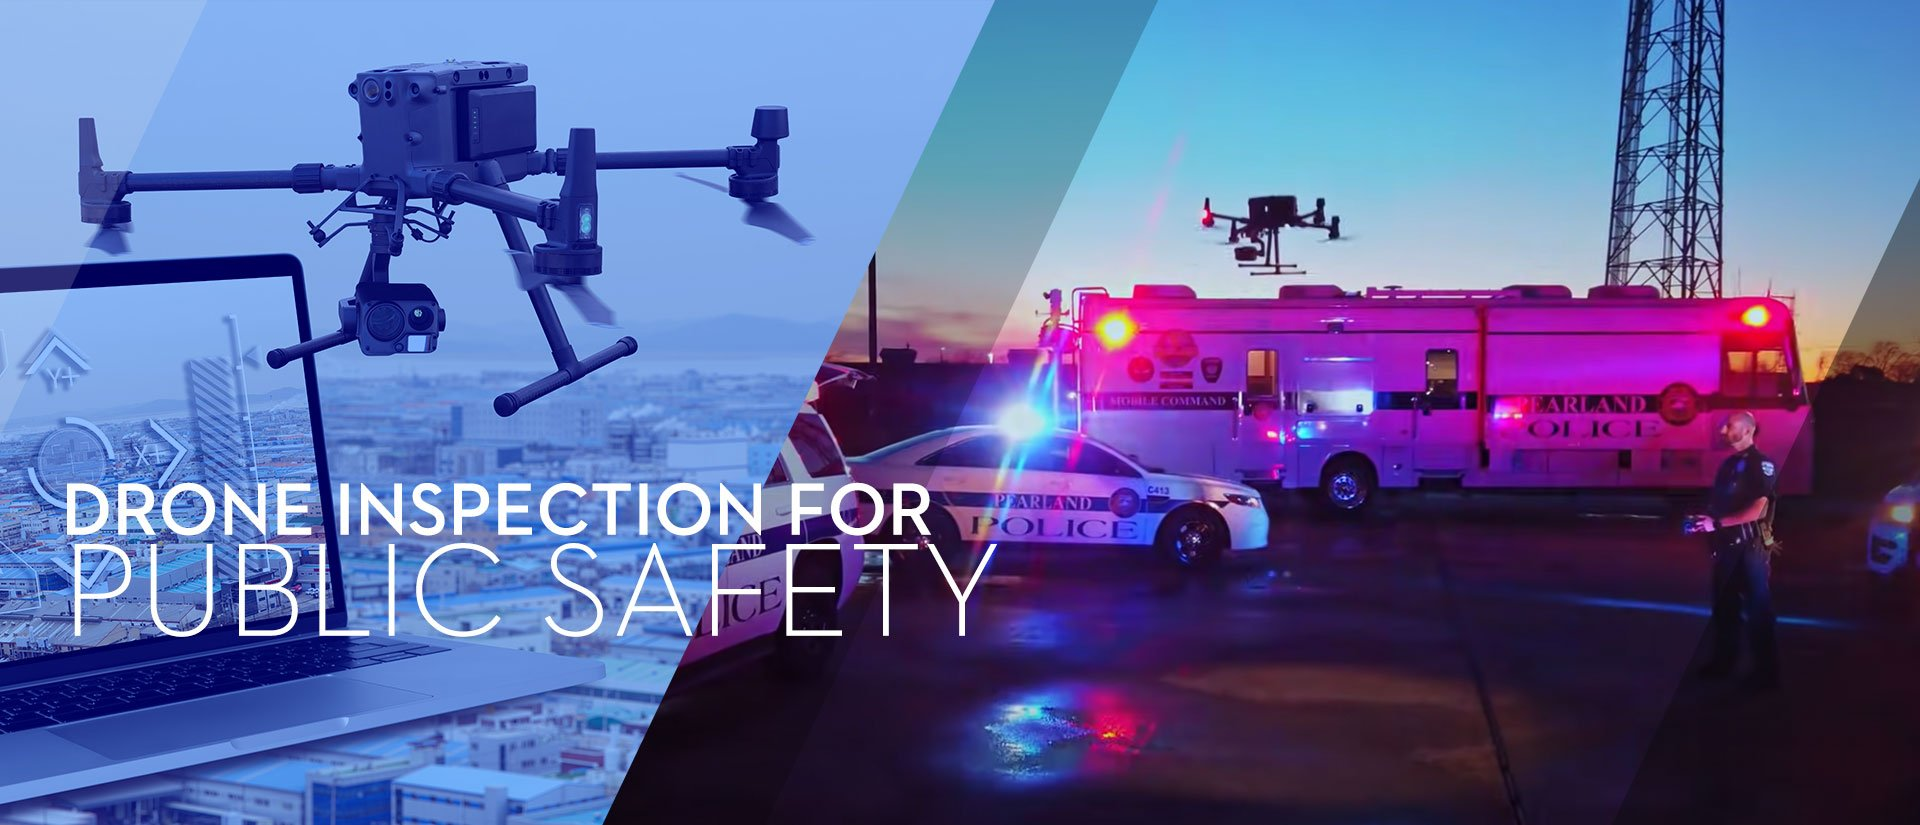
\includegraphics[width=0.45\textwidth,height=0.35\textheight]{DJI_B5}$^\dag$ 
  %\hfil
  %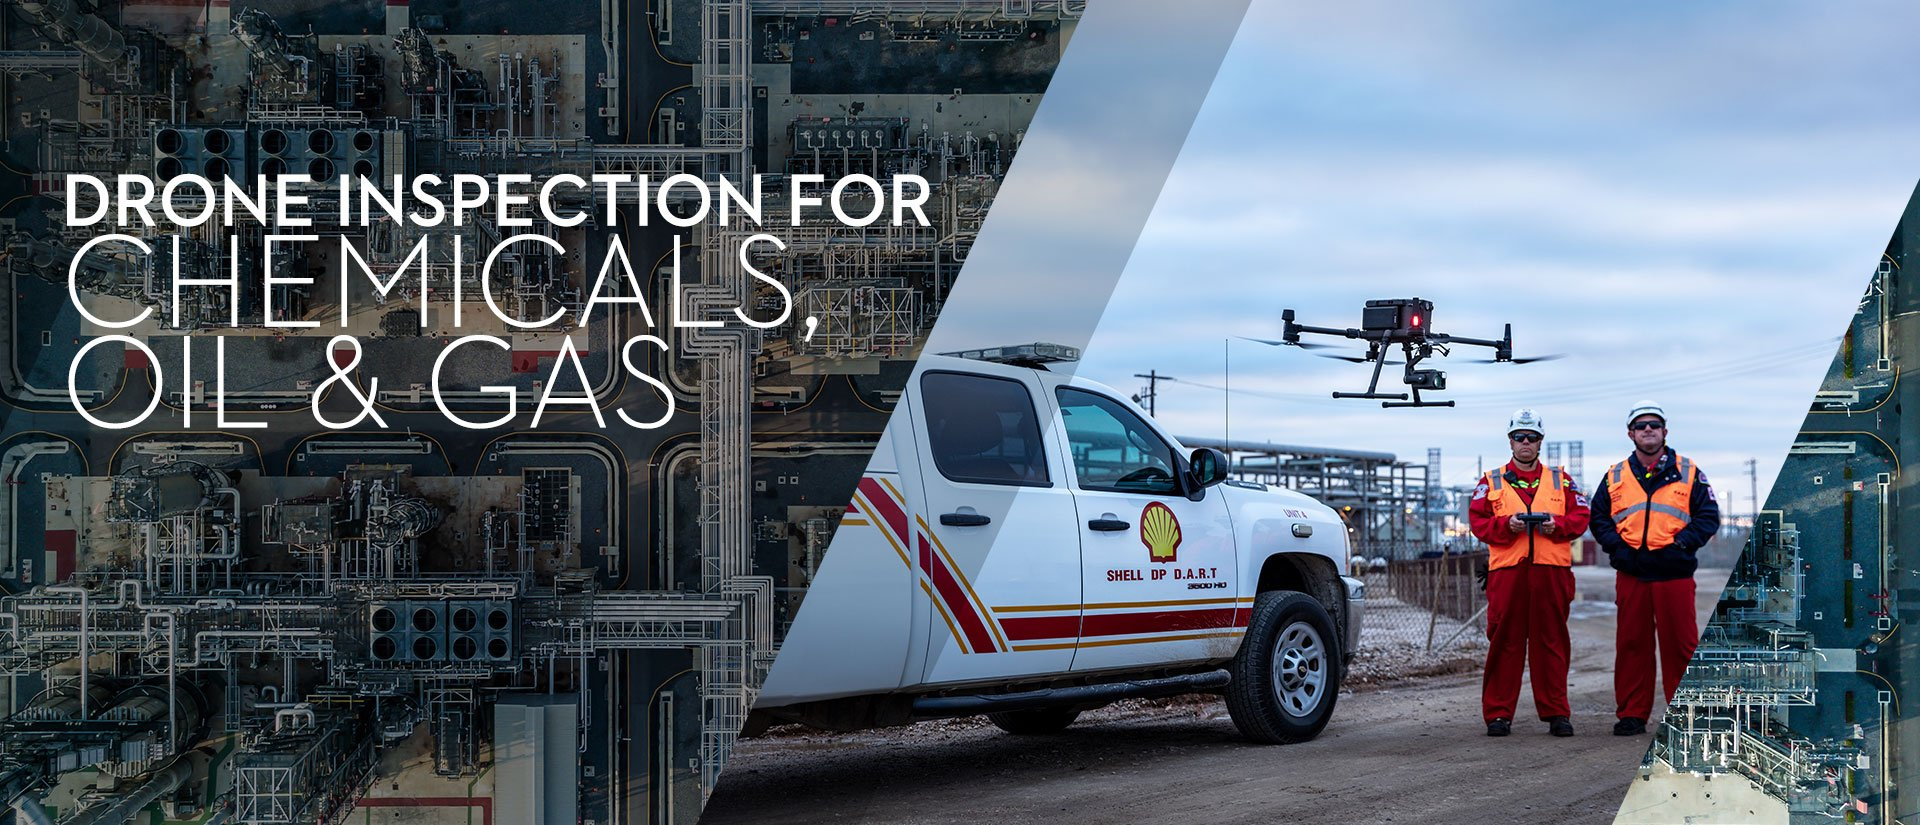
\includegraphics[width=0.45\textwidth,height=0.35\textheight]{DJI_B4}$^\dag$\\
  %\rule{0in}{1.2em}$^\dag$ \small Inspecciones con VANT basadas en los mejores casos de uso\\
  %\tiny \url{https://enterprise-insights.dji.com/blog/complete-guide-to-drone-inspections}
\end{frame}

\begin{frame}{Antecedentes}
  
  %\centering
  Principales preguntas que un robot autónomo debe responder
  \bigskip % Vertical whitespace
  \begin{itemize}
  \item ¿Dónde estoy? $\implies$ Localización 
  \item ¿A dónde voy? $\implies$ Cognición
  \item ¿Cómo llego hasta ahí? $\implies$ Planificación de trayectoria
  \end{itemize}
  \pause
  \bigskip % Vertical whitespace
  Para resolver estas preguntas, el robot debe:
  \bigskip % Vertical whitespace
  \begin{itemize}
  \item Tener un modelo del ambiente (dado, o autónomamente construido)
  \item Localizarse dentro del ambiente
  \item Planear y ejecutar los movimientos
  \end{itemize}
  
\end{frame}

\begin{frame}{Localizacion - ¿Dónde estoy?}

  \begin{minipage}{0.47\textwidth}
    \begin{itemize}
    \item \textcolor{blue}{VER}: El Robot utiliza la lectura de sus sensores para encontrarse a el mismo.
      \bigskip % Vertical whitespace
    \item \textcolor{red}{ACTUAR}: El Robot, se mueve hacia adelante
      \begin{itemize}
      \item Movimiento estimado a partir de las lecturas de la odometría.
      \item Acumulación de incertidumbre.
      \end{itemize}
      \bigskip % Vertical whitespace
    \item \textcolor{blue}{VER}: El Robot utiliza la lectura de sus sensores nuevamente para localizarse a si mismo
    \end{itemize}
  \end{minipage}
  \hspace{0.2cm}
  \begin{minipage}{0.5\textwidth}
    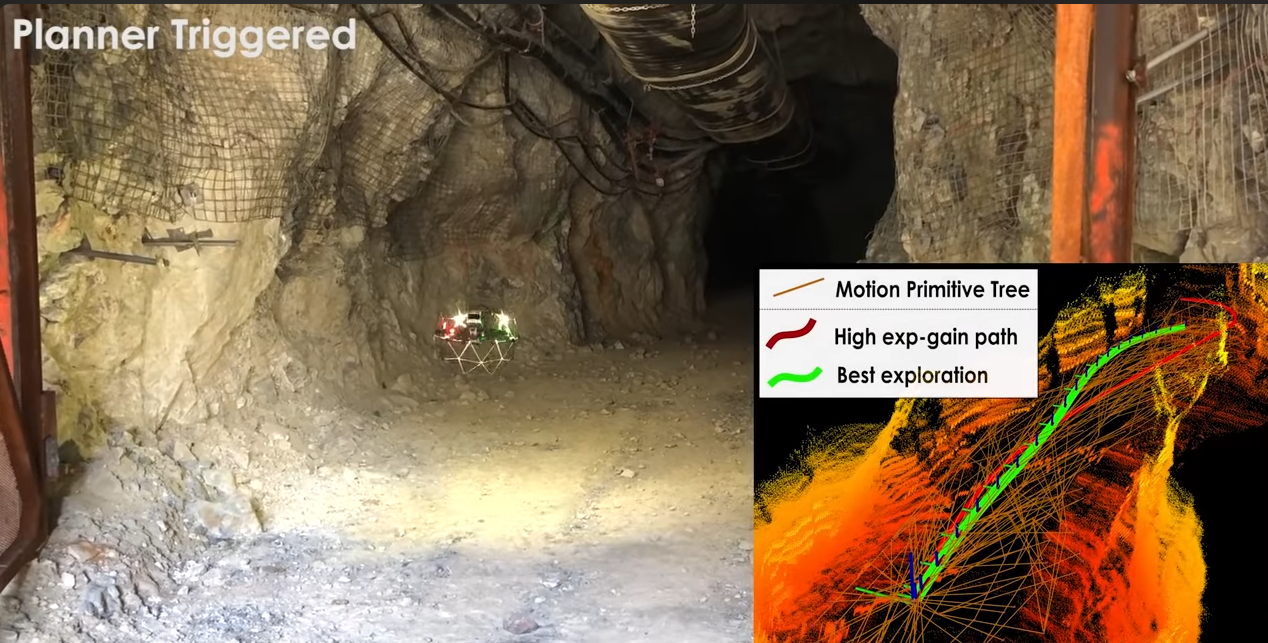
\includegraphics[width=1\textwidth]{vant_autonomo}
  \end{minipage}
    
  \bigskip % Vertical whitespace
  Belief update (Fusión de información)
\end{frame}

\begin{frame}{Cognición - ¿A dónde voy?}
  \centering
  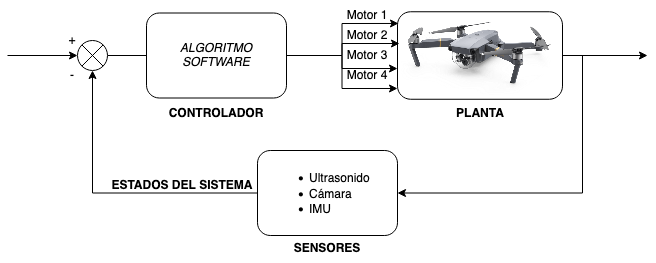
\includegraphics[width=0.65\textwidth]{control_drone.png}
\end{frame}

\begin{frame}{Planificación de trayectoria - ¿Cómo llego hasta ahí?}
  \begin{minipage}{0.47\textwidth}
    
    \begin{itemize}
    \item Planificador de trayectoria global
      \begin{itemize}
      \item Búsqueda por grafos
      \end{itemize}
      \bigskip % Vertical whitespace
    \item Planificador de trayectoria local
      \begin{itemize}
      \item Campos de potencial artifical
      \item Algoritmos Bug
      \end{itemize}
    \end{itemize}
  \end{minipage}
  \hspace{0.2cm}
  \begin{minipage}{0.5\textwidth}
    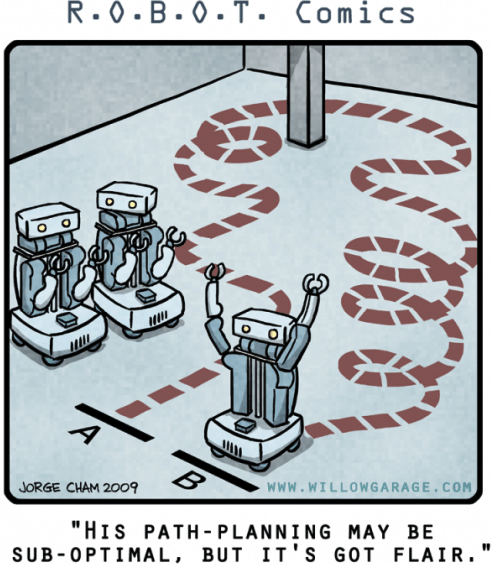
\includegraphics[width=0.6\textwidth]{img5}$^\dag$\\
  \end{minipage}
\end{frame}

%\begin{frame}{Vehículos aéreos no tripulados (VANT)}
%  \bigskip % Vertical whitespace
%  \centering
%  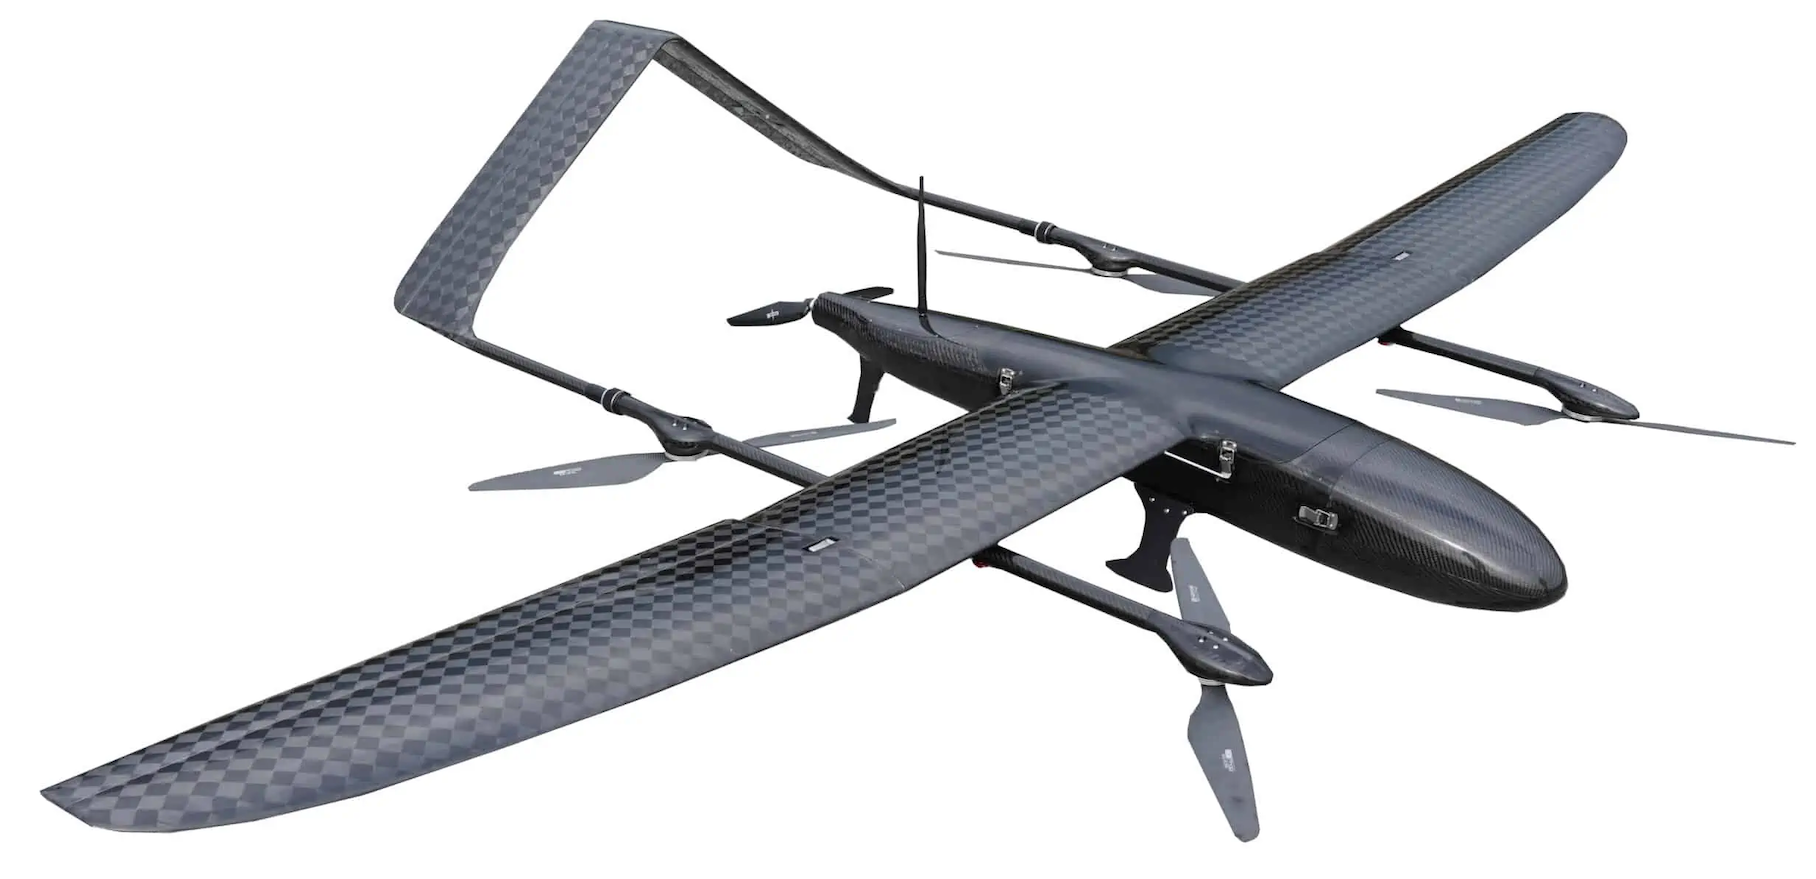
\includegraphics[width=0.45\textwidth,height=0.35\textheight]{img6}
%  \hfil
%  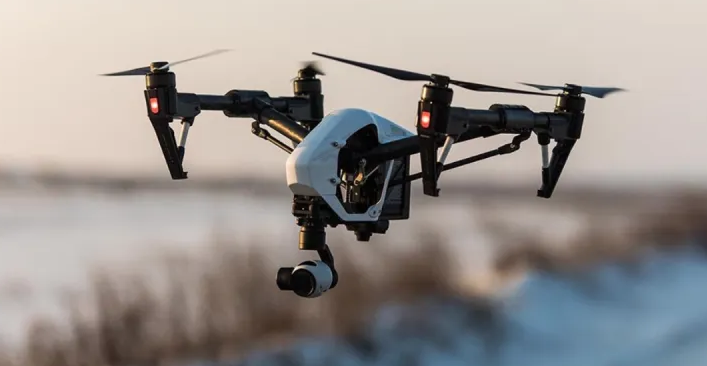
\includegraphics[width=0.45\textwidth,height=0.35\textheight]{img7}
%  \vspace{2pt}
%  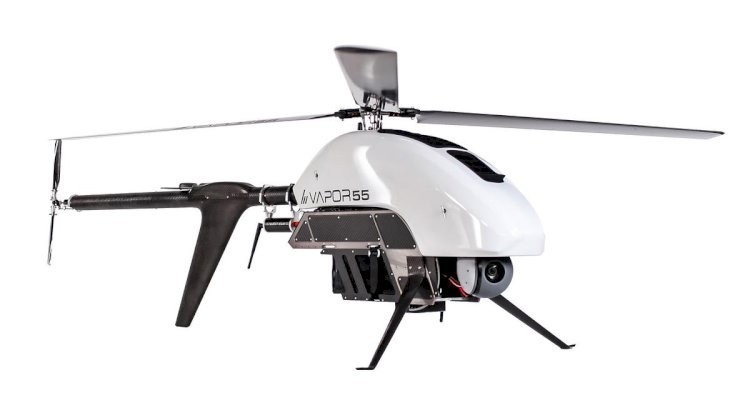
\includegraphics[width=0.45\textwidth,height=0.35\textheight]{img8.jpg}
%  \hfil
%  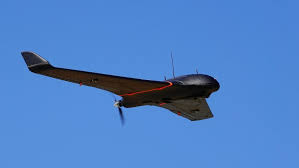
\includegraphics[width=0.45\textwidth,height=0.35\textheight]{img9.jpg}
%  \rule{0in}{1.2em} \small Clasificación VANTS \\
%  \tiny  Handbook of Unmanned Aerial Vehicles 2020
%\end{frame}
  
%\begin{frame}{Arquitectura híbrida}
%  \begin{minipage}{0.47\textwidth}
    
%    \small El robot puede reaccionar de manera rápida a estímulos del entorno, al mismo tiempo que tiene la capacidad de planificar y tomar decisiones de alto nivel.
    
%    \begin{itemize}
%    \item Adaptable al lidiar con situaciones predecibles como imprevistas.
%    \item Permite una respuesta rápida a estímulos del entorno.
%    \item Optmiza el rendimiento del robot al gestionar las tareas simples y repetitivas, liberando recursos para tareas deliberativas más complejas.
%    \item Es escalable.
%    \end{itemize}
%  \end{minipage}
%  \hspace{0.2cm}
%  \begin{minipage}{0.5\textwidth}
%    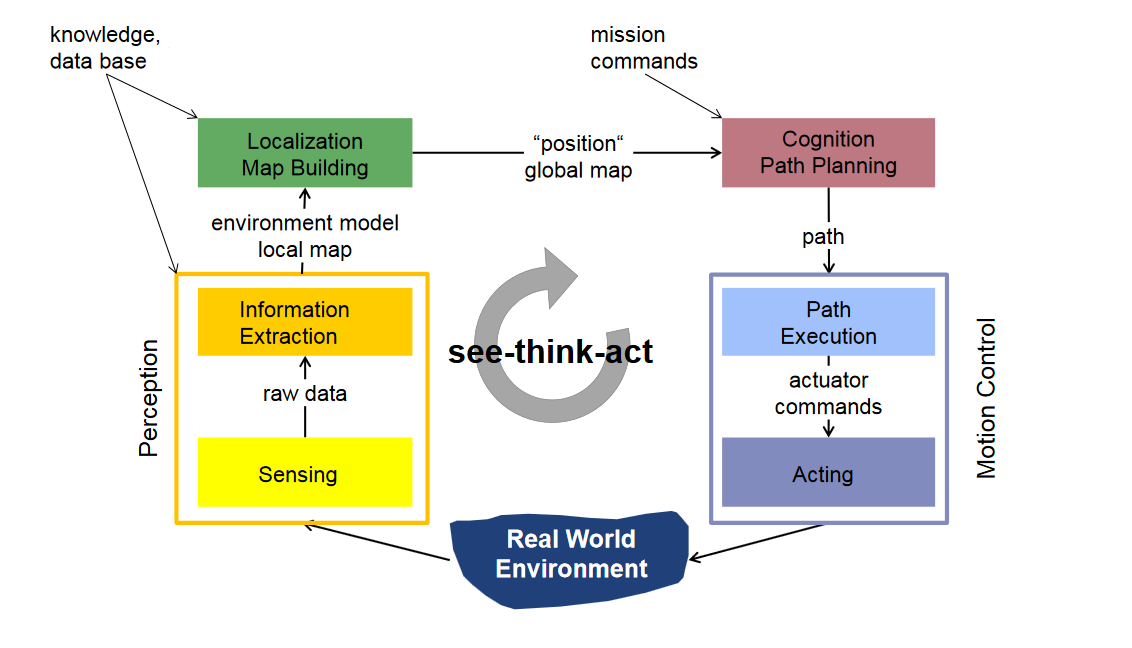
\includegraphics[width=\textwidth]{control-scheme}$^\dag$\\
%    \rule{0in}{1.2em}$^\dag$\scriptsize Ciclo See-Think-Act \\
%    \tiny ETH - Note Class Autonomous mobile robot 2015 
%  \end{minipage}
%\end{frame}

%\begin{frame}{Sistema autónomo VANT}
%  \begin{minipage}{0.47\textwidth}
    
%    \small Un sistema autónomo de un vehículo aéreo no tripulado consta de tres algoritmos.
    
%    \begin{itemize}
%    \item Generación de una representación del entorno.
%    \item Evasión de obstáculos.
%    \item Planificación de trayectorias.
%    \end{itemize}

%    \small La computadora embebida usado en un micro-VANT es de bajo rendimiento, pero su necesidad de autónomia sigue siendo la misma que un VANT de mayor tamaño.\\
%    Es necesario dotarlos de algoritmos de baja complejidad computacional.
    
%  \end{minipage}
%  \hspace{0.2cm}
%  \begin{minipage}{0.5\textwidth}
%    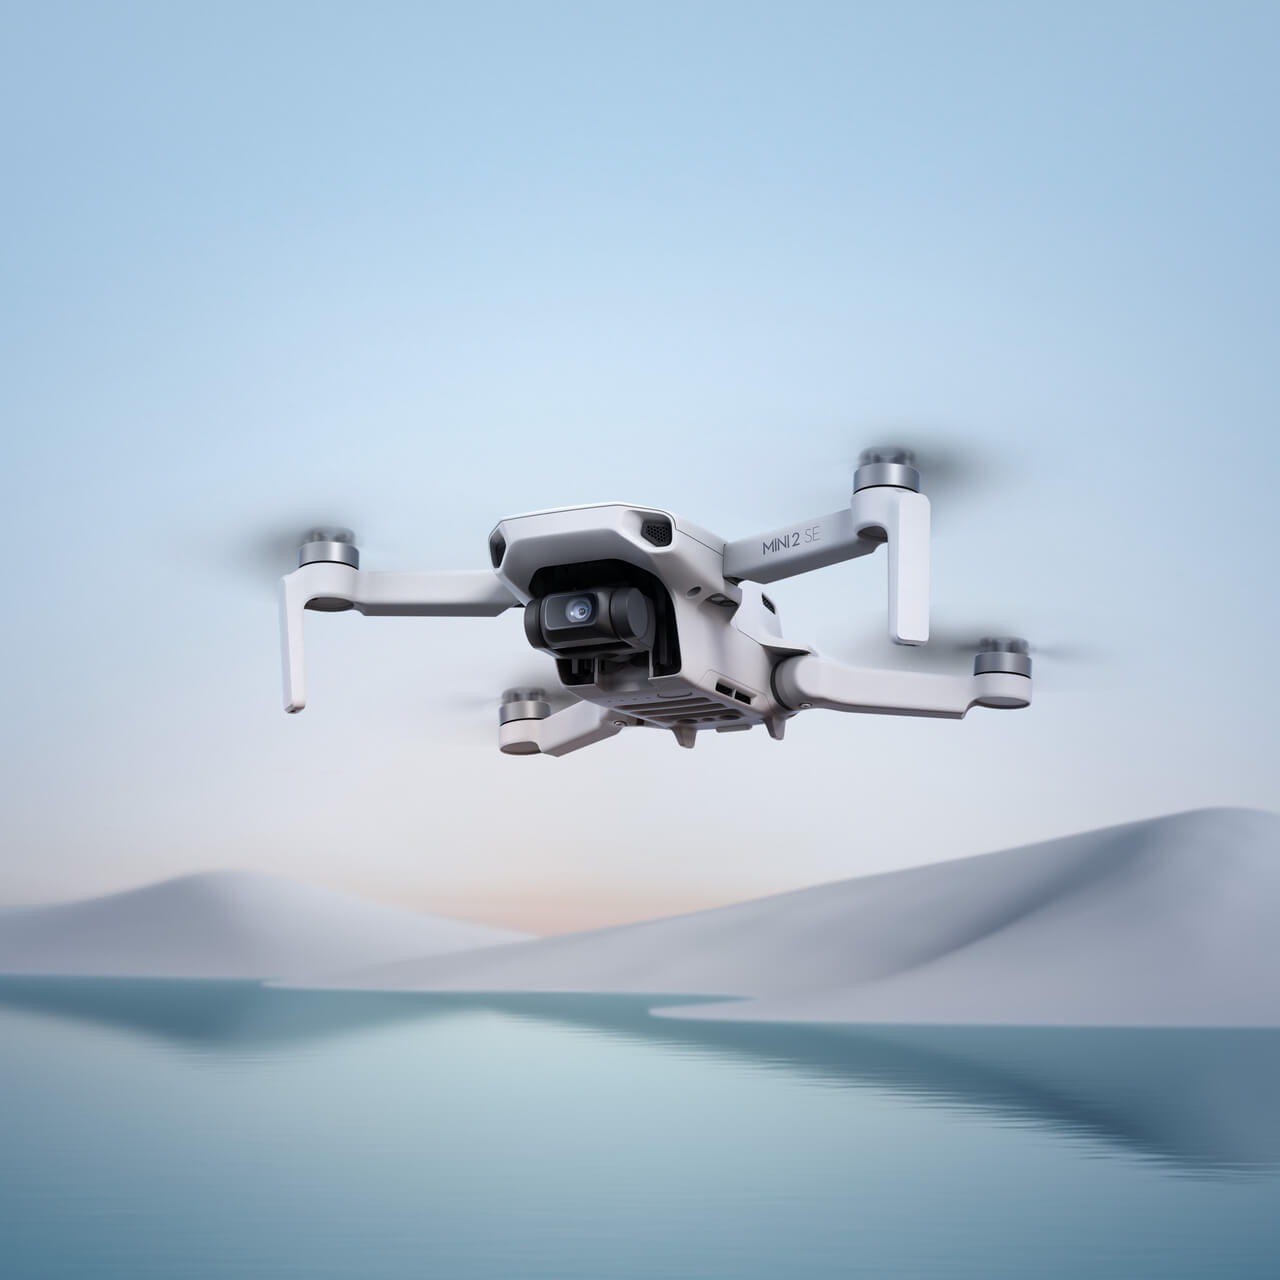
\includegraphics[width=\textwidth]{ultra.jpg}
%  \end{minipage}
%\end{frame}

%\begin{frame}{Generación de mapas}
%  \bigskip % Vertical whitespace
  %\centering
%  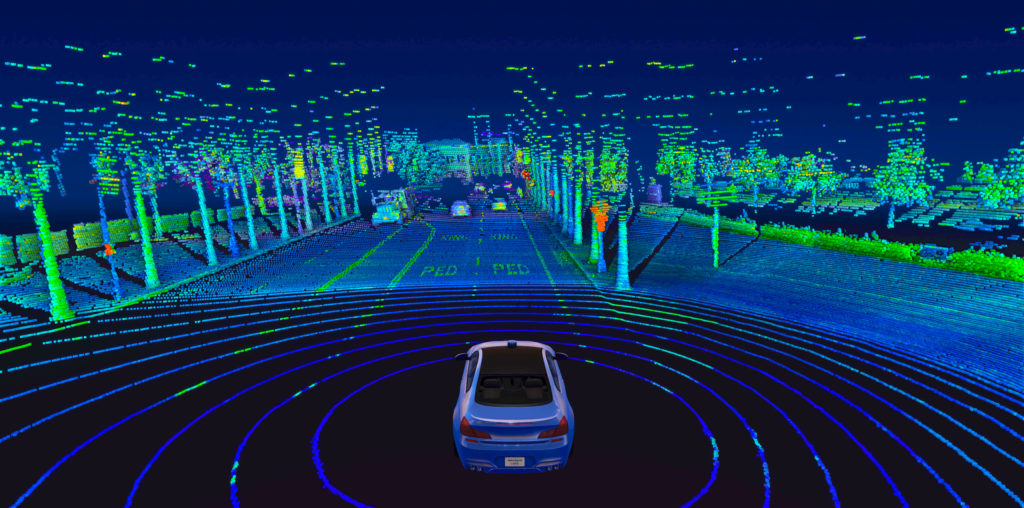
\includegraphics[width=0.45\textwidth,height=0.35\textheight]{map3d.jpg}$^\dag$
%  \hfil
%  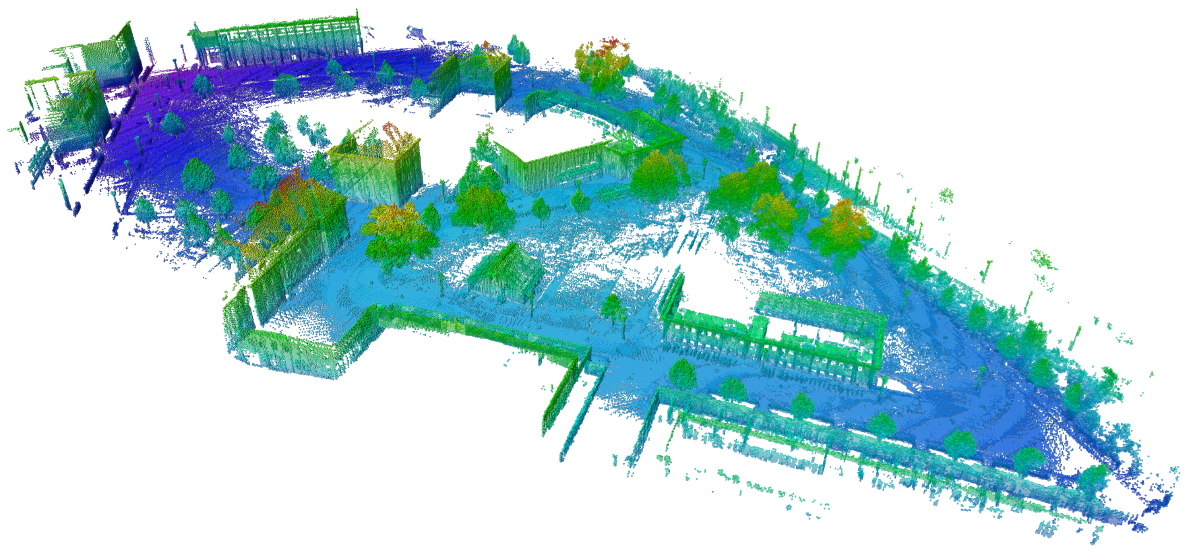
\includegraphics[width=0.45\textwidth,height=0.35\textheight]{map3d_2}$^\dag$
%  \vspace{2pt}\\
%  \bigskip % Vertical whitespace
%  Es la construcción de un mapa del entorno, realizada por un robot, utilizando información espacial obtenida durante el paso del tiempo. [\citeauthor{Wallgrn2010} 2010]\\
%  \bigskip % Vertical whitespace
%  Fuentes de información:
%  \begin{itemize}
%  \item Escáners láser tipo LIDAR.
%  \item Cámaras RGBD.
%  \end{itemize}  

  %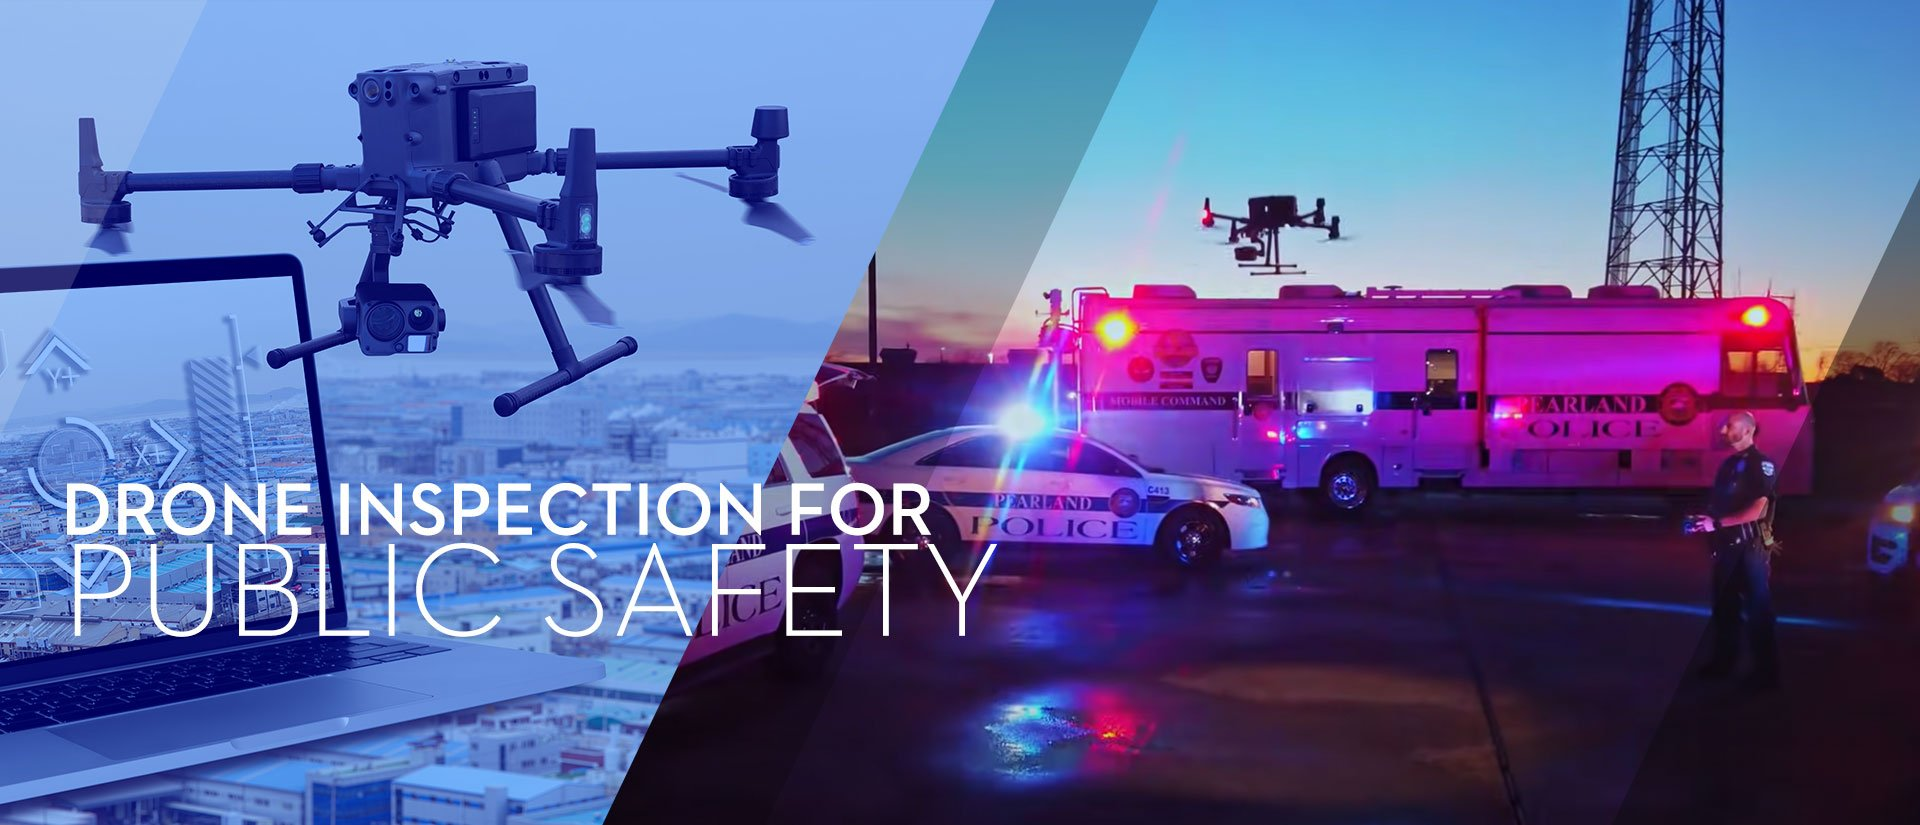
\includegraphics[width=0.45\textwidth,height=0.35\textheight]{DJI_B5}$^\dag$ 
  %\hfil
  %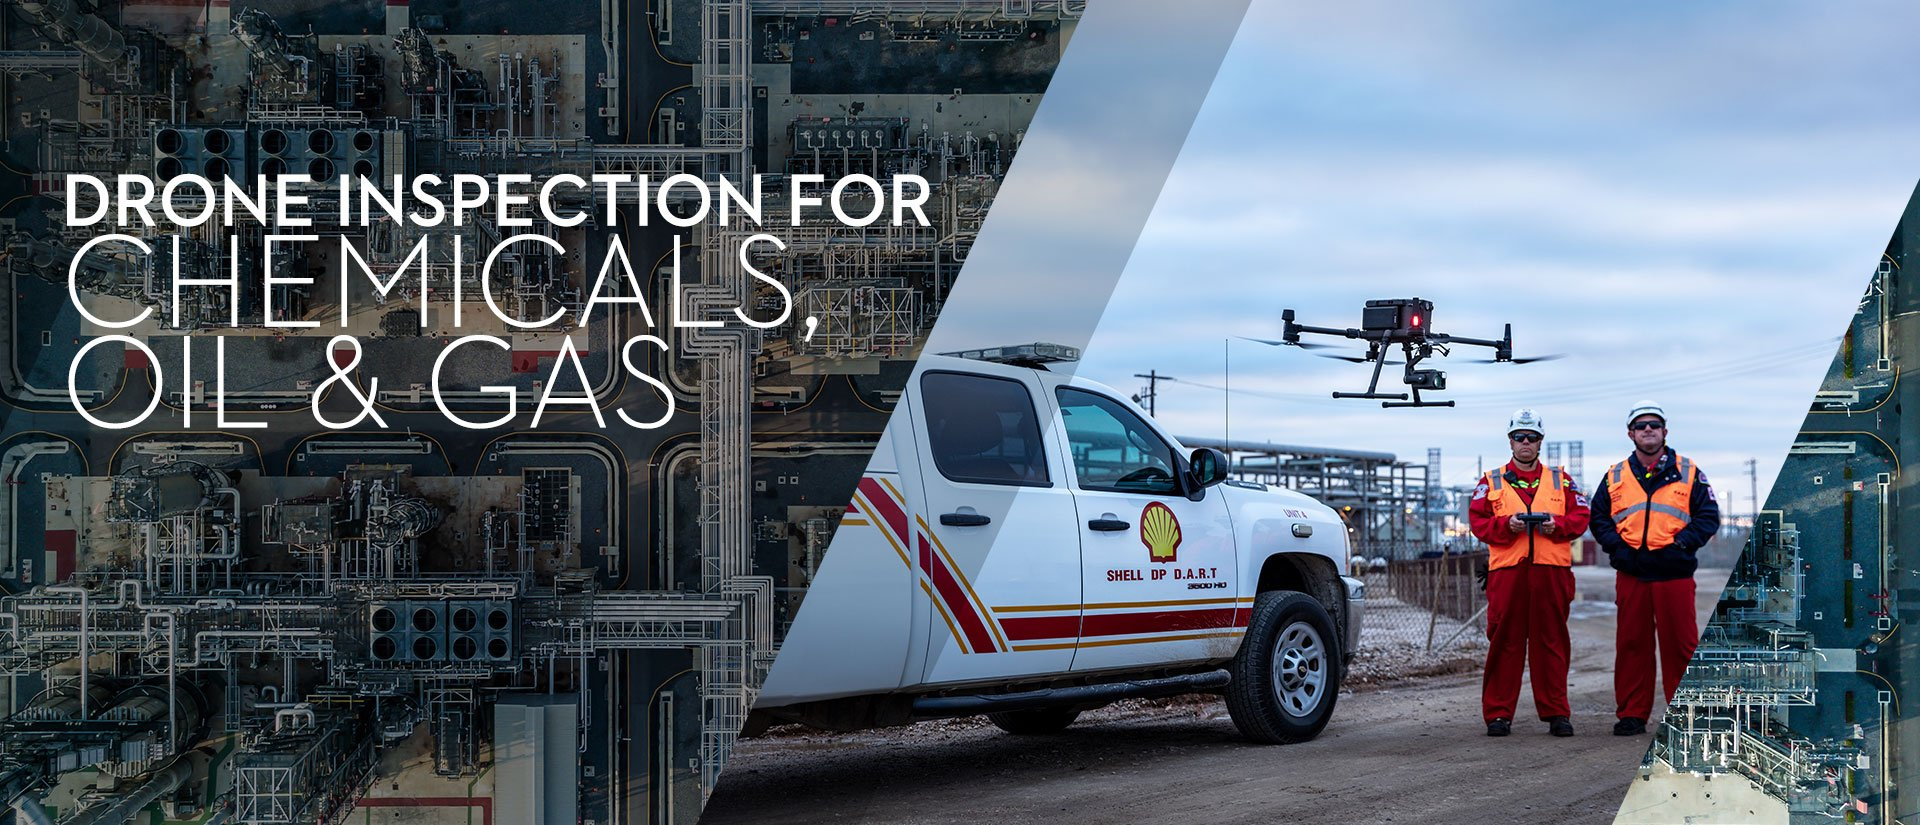
\includegraphics[width=0.45\textwidth,height=0.35\textheight]{DJI_B4}$^\dag$\\
  %\rule{0in}{1.2em}$^\dag$ \small Inspecciones con VANT basadas en los mejores casos de uso\\
  %\tiny \url{https://enterprise-insights.dji.com/blog/complete-guide-to-drone-inspections}
%\end{frame}

%\begin{frame}{Representacion 3D}
%  \bigskip % Vertical whitespace
  %\centering
%  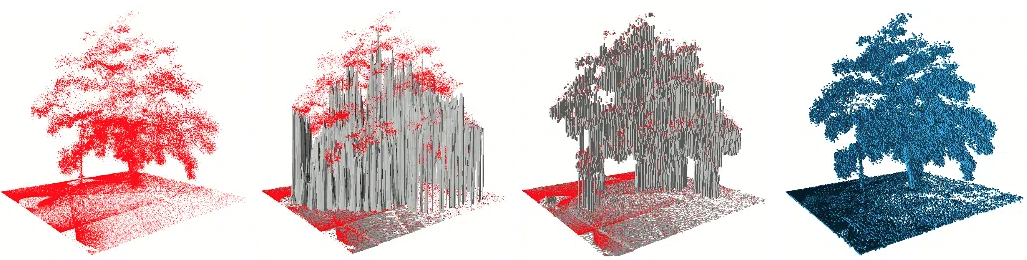
\includegraphics[width=1\textwidth,height=0.35\textheight]{img4}\footnotemark
%  \vspace{2pt}\\
%  \bigskip % Vertical whitespace
  
%  \begin{itemize}
%  \item Nube de puntos.
%  \item Mapa de elevación.
%  \item Superficies multi-nivel.
%  \item Octrees.
%  \end{itemize}
%  \footnotetext{OctoMap: An Efficient Probabilistic 3D Mapping Framework Based on Octrees [\cite{hornung13auro}]}
  
%\end{frame}

%\begin{frame}{Planificación de movimiento}
  
  %\centering
  %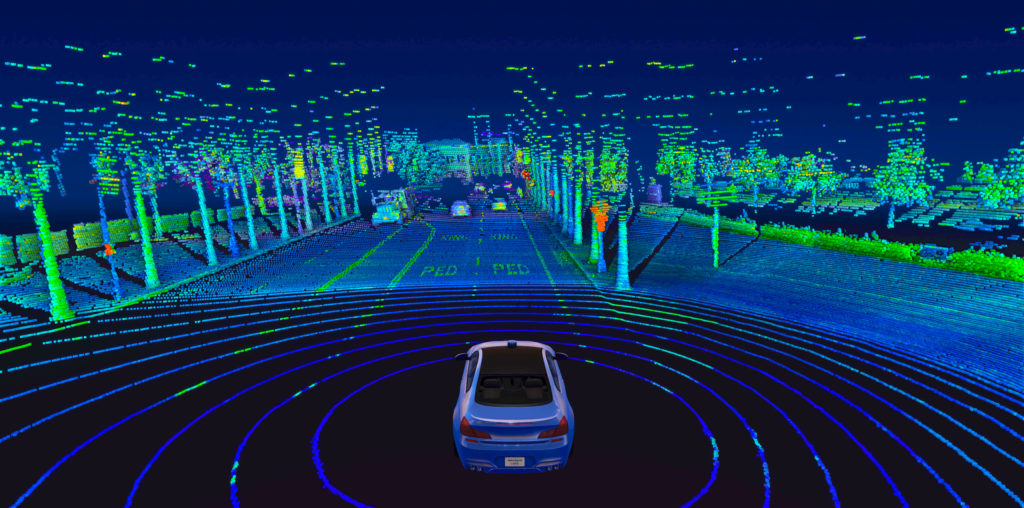
\includegraphics[width=0.45\textwidth,height=0.35\textheight]{map3d.jpg}$^\dag$
  %\hfil
  %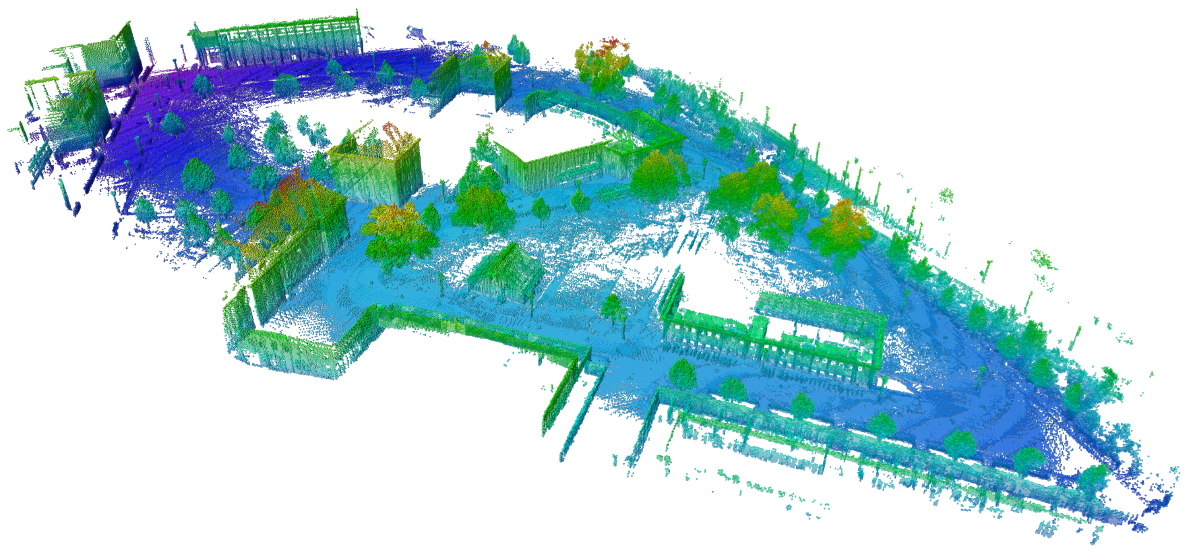
\includegraphics[width=0.45\textwidth,height=0.35\textheight]{map3d_2}$^\dag$
  %\vspace{2pt}\\
  %\bigskip % Vertical whitespace
%  Indica a un robot como moverse de un punto a otro en su entorno. Implica la generación de trayectorias y movimientos que permiten a los robots cumplir sus tareas o alcanzar sus objetivos mientras evitan obstáculos \footnotemark.\\
%  \bigskip % Vertical whitespace
%  \addvspace{\medskipamount}
%  \noindent
%  \begin{tabularx}{\linewidth}{ @{} X X @{} }
%    Por Grafos
    
%    \begin{itemize}
%    \item Grafos de visibilidad. 
%    \item Diagramas de Voronoi.
%    \item Descomposición por celdas.
%    \item Consulta única (RRT)
%    \item Consulta múltiple (PRM)
%    \end{itemize} &

%    Algoritmos
    
%    \begin{itemize}
%    \item BFS, DFS
%    \item A*, D*
%    \item Dijkstra
%    \end{itemize}
%  \end{tabularx}
%  \footnotetext{Different Cell Decomposition Path Planning Methods for Unmanned Air Vehicles A Review [\cite{Debnath2020}]}
%\end{frame}

\begin{frame}{Motivaciones}
  \begin{minipage}{0.47\textwidth}

    \small La meta de este trabajo es la creación de una estrategia para la exploración de ambientes desconocidos de manera coordinada con múltiples vehículos aéreos no tripulados (VANTS).
    \bigskip % Vertical whitespace
    \begin{itemize}
    %\item Exploración con algoritmos de baja complejidad computacional.
    \item Búsqueda y rescate.
    \item Seguridad e Inspección
    \end{itemize}
  \end{minipage}
  \hspace{0.2cm}
  \begin{minipage}{0.5\textwidth}
    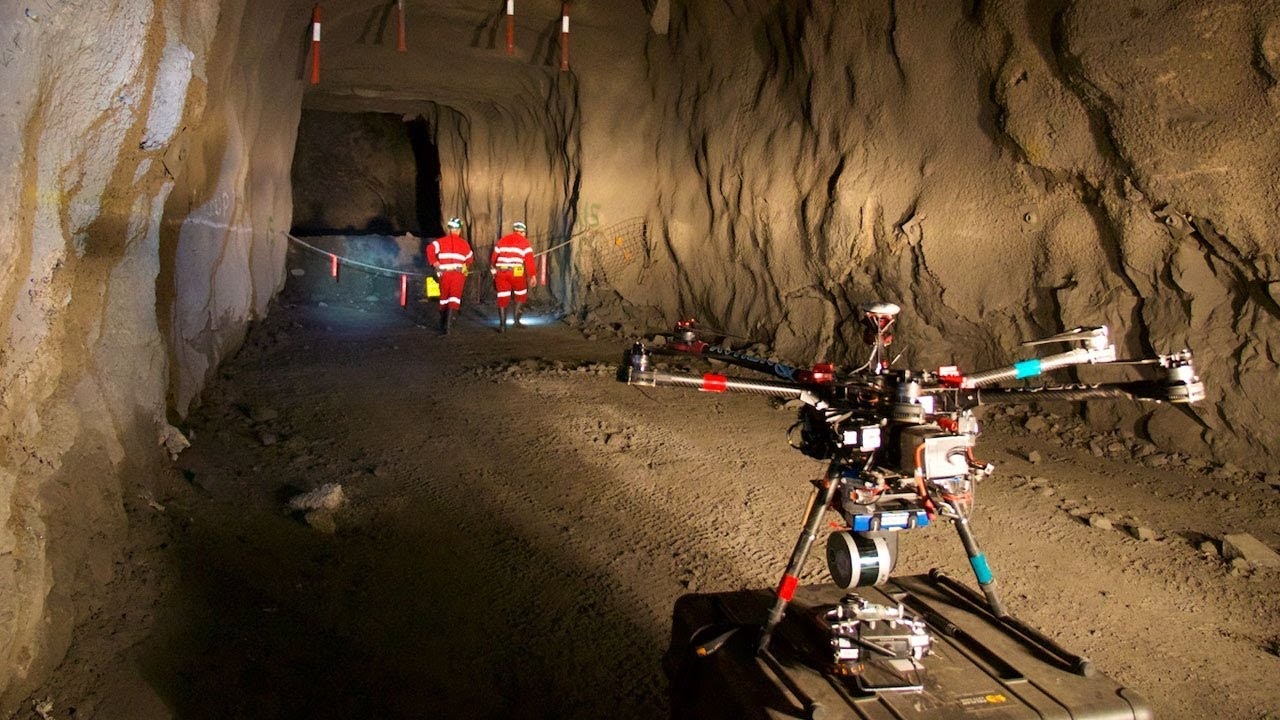
\includegraphics[width=\textwidth]{maxresdefault.jpg}$^\dag$\\
      \rule{0in}{1.2em}$^\dag$\scriptsize Ilustración Drone en Mina \\
      \tiny \url{https://dronevideos.com/} 
  \end{minipage}
\end{frame}

\section{Planteamiento del problema}
\begin{frame}
  \frametitle{Planteamiento del problema}
  %\begin{columns}
  %  \column{0.5\textwidth}
  \justifying
  \small Dado un volumen de interés desconocido en un espacio cerrado que se desea explorar denotada como $\mathcal{S}$, tal que $\mathcal{S} \subset \mathbb{R}^{3}$.\\
  Encontrar y repartir rutas libres de colisiones para un conjunto de VANTS denotado como $\mathcal{V} = \{\mathcal{V}_{1},\mathcal{V}_{2},\mathcal{V}_{3},...,\mathcal{V}_{n}\}$ siendo $n$ el número total de VANTS disponibles, comenzando cada uno en un estado inicial conocido denotados como $q = \{q_{1},q_{2},q_{3},...,q_{n}\}$, y terminando en una configuración que maximice la localización del VANT y exactitud en la construcción del mapa.\\

  La representación del volumen a explorar se utiliza un mapa de ocupación que se obtiene dividiendo el volumen en volumenes cúbicos (voxel) que puede tomar los valores de libre, ocupado y desconocido o no explorado de notados como $v_{libre}$, $v_{ocup}$, $v_{desc}$ con lecturas a partir de los valores de una cámara RGB-D basada en un modelo de ocupación probabilístico.\\

  \bigskip % Vertical whitespace
  El problema se basa en la propuesta de una estrategia que incluya las habilidades de autonomía, para tareas de exploración de forma coordinada dividiendo la carga de trabajo de exploración entre el grupo de una forma descentralizada.\\
  
  %Para lograr una exploraci\'{o}n eficiente y completa con un tiempo y recursos m\'{i}nimos, el problema requiere la creaci\'{o}n de algoritmos y t\'{e}cnicas de optimizaci\'{o}n.\\
    
  %\pause
  
  
   % \column{0.5\textwidth}\\
   % \pause
   % \centering
   % \small Retos multi-VANT
   % \begin{itemize}
   % \small \item Coordinación% - Establecer comunicación efectiva entre los múltiples VANTs. Intercambiar información relevante. Tener baja latencia en su comunicación.
   % \small \item Planificación% - Los VANTs deben coordinar sus movimientos para evitar colisiones y lograr una cobertura eficiente del área objetivo.
   % \small \item Asignación de tareas% - Se busca evitar la duplicación de esfuerzos optimizando el uso de recursos disponibles.
   % \end{itemize}
   %\end{columns}
\end{frame}

\begin{frame}{Preguntas de investigación}
  
  %\pause
  \begin{itemize}

  \item ¿Qué mecanismos de coordinación existen dentro de la literatura de teoría de juegos podrían ayudar en resolver el problema de exploración multi-VANT?
  \item ¿Es posible que el uso de una estructura de datos como octree para representar la ocupación de un volumen, sea más eficiente que una representación usando una matriz cúbica?
    %\pause
  %\item ¿Qué efectiva será en seguir una estrategia de exploración basada en asignación de tareas en comparación con los resultados reportados en la literatura?
    %\pause
  \item ¿Qué características de la dinámica del robot se deben considerar en el simulador, para que los resultados en el mundo real se aproximen a los del simulador?
    
  \end{itemize}
\end{frame}

\section{Hipótesis y Objetivos}

\begin{frame}{Hipótesis}

  Una estrategia de exploración con un efoque en coordinación y asignación de tareas, en combinación con una arquitectura de software (que resuelve los problemas de planificación de rutas, evasión de obstáculos y localización) puede mejorar la tarea de exploración de múltiples VANTS en entornos desconocidos tomado un enfoque descentralizado.
  
  %La implementación de una estrategia de exploración coordinada utilizando múltiples vehículos aéreos no tripulados (multi-VANT) en ambientes sin señal GPS, permitirá obtener mejores resultados en comparación con la exploración individual (mono-VANT). Esta coordinación eficiente se traducirá en una reducción del tiempo y los recursos necesarios para completar la exploración, así como en una mayor cobertura del área de interés. Además, se espera que la exploración coordinada multi-VANT mejore la calidad de los datos recopilados, lo que permitirá tomar decisiones más informadas y eficaces en diversos campos, como la cartografía, la vigilancia, el monitoreo y la respuesta a desastres naturales.
  
  %La implementación de una arquitectura descentralizada integrada de algoritmos para la detección y evasión de obstáculos, toma de decisiones, navegación e inteligencia colectiva para los múltiples VANTS. Así como un enfoque de fusión de datos que integre la información de los sensores de los múltiples VANTS, mejorará la efectividad y conducirá a mejores resultados de exploración en entornos dinámicos e inciertos, incluida una mayor cobertura del área explorada, una mejor recopilación de datos en comparación con un enfoque de un solo VANT.
  
\end{frame}

\begin{frame}{Objetivos generales y específicos del proyecto}
  %\frametitle
  \begin{enumerate}
    %\item<1-> General \\
    \item General \\
    \bigskip
    Desarrollar una estrategia de exploración descentralizada que permita resolver los problemas de coordinación para múltiples VANTS en ambientes desconocidos.
    \pause
    \bigskip
    % \item<2-> Particulares\\
    \item Particulares\\
    
    \begin{itemize}
    \item Desarrollar una arquitectura de software que resuelva los problemas de autonomía para un VANT (localización, manejo de mapas y navegación).
    \item Crear un mecanismo de coordinación que asigne trayectorias libres de colisiones para la tarea de exploración.
    \item Realizar pruebas y simulaciones de la solución propuesta en entornos complejos, analizando métricas como tiempo de exploración y cobertura del área de interés.
    \end{itemize}
  \end{enumerate}
\end{frame}

%Explicar con el cronograma
\section{Metodología}
\begin{frame}{Metodología}
%\small Siguiendo los objetivos anteriores, la metodolog\'{i}a propuesta se divide en tres etapas, que comenzaron en septiembre del 2023 y terminarán en agosto de 2024. A continuaci\'{o}n se detallan cada una de las actividades que se plantean realizar en cada etapa.

%\small \textbf{Etapa 1. An\'{a}lisis y dise\~{n}o de la soluci\'{o}n propuesta}\\
%\small Esta etapa comprende la revisi\'{o}n de la literatura de manera m\'{a}s completa, que permita contar con la informaci\'{o}n necesaria para la elecci\'{o}n de los mejores algoritmos para abordar cada una de las problem\'{a}ticas asociadas con la coordinaci\'{o}n de múltiples robots en tareas de exploración, detectando áreas de oportunidad para el desarrollo de una estrategia descentralizada de coordinación. \\
%\bigskip
%\small \textbf{Etapa 2. Implementaci\'{o}n y validaci\'{o}n}\\
%\small Esta etapa se centra en el desarrollo e implementaci\'{o}n del dise\~{n}o de la arquitectura de software para la coordinaci\'{o}n multi-VANT, utilizando una herramienta de simulación de robots de libre acceso, cumpliendo estándares de modularidad de diseño.\\
%\bigskip
%\small \textbf{Etapa 3. Evaluaci\'{o}n experimental, resultados y conclusiones}\\
%\small Partiendo del prototipo y las simulaciones desarrolladas en la etapa anterior, en esta etapa se realizan todas las actividades relacionadas con la evaluación, compilación y análisis de los resultados.
  
%\begin{frame}{Metodología/Cronograma}
  \begin{figure}
    \centering
    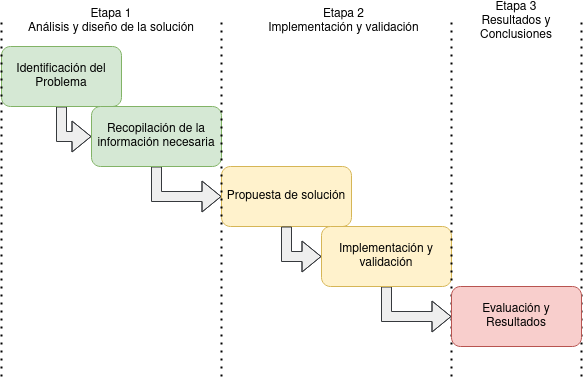
\includegraphics[width=10cm]{metodologia}
  \end{figure}
\end{frame}

\section{Cronograma}
\begin{frame}{Cronograma}
\tiny 

\hspace{0.0cm}\begin{minipage}{7cm}
  \noindent\begin{tabular}{|p{0.8\textwidth}*{12}{|p{0.040\textwidth}}|}
  % The top line
  %\diagbox[width=12.5em]{Actividades}{Cuatrimestres}
  \hline
  & \multicolumn{4}{c|}{\textbf{Cuatrimestre 1}} 
  & \multicolumn{4}{c|}{\textbf{Cuatrimestre 2}}
  & \multicolumn{4}{c|}{\textbf{Cuatrimestre 3}}\\
  \hline
  % The second line, with its five years of four quarters
  %\textcolor{black}{\textbf{Etapas}}
  \rpt[3]{& 1 & 2 & 3 & 4} \\
  \hline
  \rowcolor{black!5}{\textbf{Etapa 1}}\\
  % using the on macro to fill in twenty cells as `on'
  %\specialcell{Actividad 1\\espacio}        \on[0] \off[12] \\
%Actividad 1    \on[0] \off[12]\\
\hline
\textbf{E1.A1.} Revisi\'{o}n literatura relevante
%en exploraci\'{o}n multi-VANT, estrategias de exploraci\'{o}n, algoritmos de coordinaci\'{o}n y evaci\'{o}n de obst\'{a}culos
\on[12] \\
\hline
%\textbf{E1.A2.} Evaluaci\'{o}n de aptitudes\footnote{Evaluaci\'{o}n a partir de los nuevos trabajos}     \on[12] \\
%\hline
\textbf{E1.A2.} Selecci\'{o}n de algoritmos \on[2] \off[10] \\
\hline
\textbf{E1.A3.} Dise\~{n}o de la arquitectura de software \off[1] \on[3] \off[8] \\
\hline
\textbf{E1.A4.} Documentaci\'{o}n Etapa 1 \on[4]  \off[8] \\
\hline
\textbf{E1.A5.} Revisi\'{o}n de tesis Etapa 1 \off[3] \on[1]  \off[8] \\
\hline
% using the on macro followed by the off macro
\rowcolor{black!5}{\textbf{Etapa 2}}\\
\hline
\textbf{E2.A1.} Selecci\'{o}n Simulador
\on[1]  \off[11] \\
\hline
\textbf{E2.A2.} Visualizaci\'{o}n de datos
\off[1] \on[2]  \off[9] \\
\hline
\textbf{E2.A3.} Control de desplazamientos
\off[2] \on[2]  \off[8] \\
\hline
\textbf{E2.A4.} Desarrollo de algoritmo de exploraci\'{o}n
\off[3] \on[2] \off[7] \\
\hline
\textbf{E2.A5.} Implementaci\'{o}n y simulaci\'{o}n
\off[3] \on[2] \off[7] \\
\hline
%\textbf{E2.A6.} Simulaci\'{o}n un solo VANT
%\off[4] \on[1] \off[7] \\
%\hline
\textbf{E2.A6.} Desarrollo de coordinaci\'{o}n
\off[4] \on[3] \off[5] \\
\hline
\textbf{E2.A7.} Implementaci\'{o}n y sumulaci\'{o}n
\off[6] \on[2] \off[4] \\
\hline
%\textbf{E2.A9.} Simulaci\'{o}n multi-VANT
%\off[6] \on[1] \off[5] \\
%\hline
\textbf{E2.A8.} Documentaci\'{o}n Etapa 2
\off[4] \on[4] \off[4] \\
\hline
\textbf{E2.A9.} Revisi\'{o}n de tesis Etapa 2
\off[7] \on[1] \off[4] \\
\hline
\rowcolor{black!5}{\textbf{Etapa 3}}\\
\hline
\textbf{E3.A1.} Experimentaci\'{o}n de soluci\'{o}n
\off[7]  \on[3] \off[2] \\
\hline
\textbf{E3.A2.} Recopilaci\'{o}n resultados
\off[9]  \on[1] \off[2] \\
\hline
\textbf{E3.A3.} Documentaci\'{o}n Etapa 3
\off[8] \on[3] \off[1] \\
\hline
\textbf{E3.A4.} Revisi\'{o}n de tesis
\off[10] \on[2] \\
\hline
\textbf{E3.A5.} Divulgaci\'{o}n
\off[5]  \on[7] \\
\hline
\textbf{E3.A6.} Proceso de titulaci\'{o}n
\off[11] \on\\
\hline
\end{tabular}
\end{minipage}

\end{frame}

\begin{frame}{Estrategia}
  
  \begin{minipage}{0.67\textwidth}
    \begin{itemize}
    \item[] \textcolor{teal}{Buscar que cada VANT se dirija hacia las fronteras más cercanas tratando de minimizar las distancias recorridas.}
      \bigskip % Vertical whitespace
    \item[] \textcolor{red}{Buscar la separación de los VANTS con la finalidad de minimizar el trabajo redundante y la interferencia entre ellos.}
      \bigskip % Vertical whitespace
    \item[] \textcolor{blue}{Mantener los VANTS en comunicación con los demás miembros del equipo actualizados y en caso de falla de algún VANT evitar que se pierda la información.}
    \end{itemize}
  \end{minipage}
  \hspace{0.6cm}
  \begin{minipage}{0.2\textwidth}
    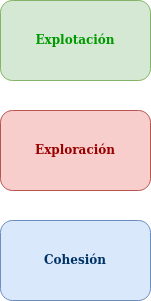
\includegraphics[width=1\textwidth]{estrategia}
  \end{minipage}
  
\end{frame}

\begin{frame}{Algoritmos}
  
  \begin{minipage}{0.47\textwidth}
    
    \begin{itemize}
      %\item Exploración con algoritmos de baja complejidad computacional.
    \item \small PRM 
    \item \small RGB-D $\implies$ Voxels $\implies$ Octomap
    \item \small Estrategia coordinada y basada en fronteras que aproveche la dinámica del VANT para obtener movimientos agresivos.
    \end{itemize}
  \end{minipage}
  \hspace{0.1cm}
  \begin{minipage}{0.5\textwidth}
    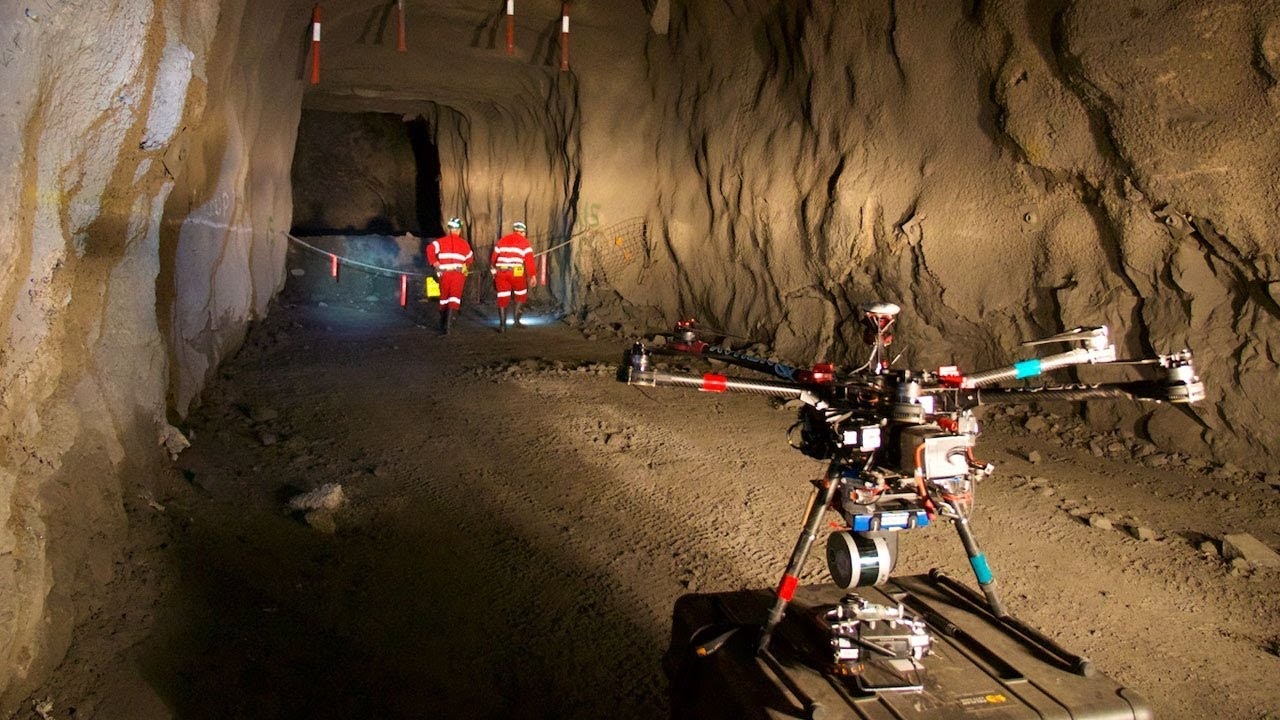
\includegraphics[width=\textwidth]{maxresdefault.jpg}$^\dag$\\
    \rule{0in}{1.2em}$^\dag$\scriptsize Ilustración Drone en Mina \\
    \tiny \url{https://dronevideos.com/} 
  \end{minipage}
  
\end{frame}

\begin{frame}{Arquitectura}
  \begin{figure}
    \centering
    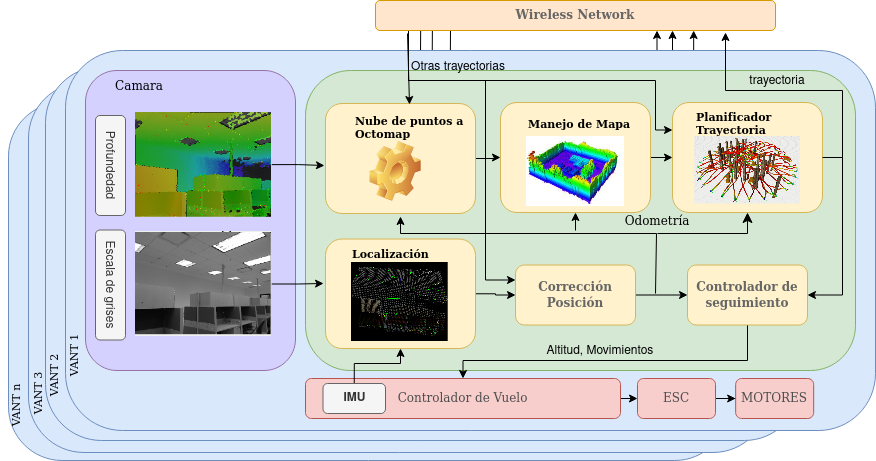
\includegraphics[width=15cm]{arquitectura}
  \end{figure}
\end{frame}

\begin{frame}{Simulador}
  \begin{figure}
    \centering
    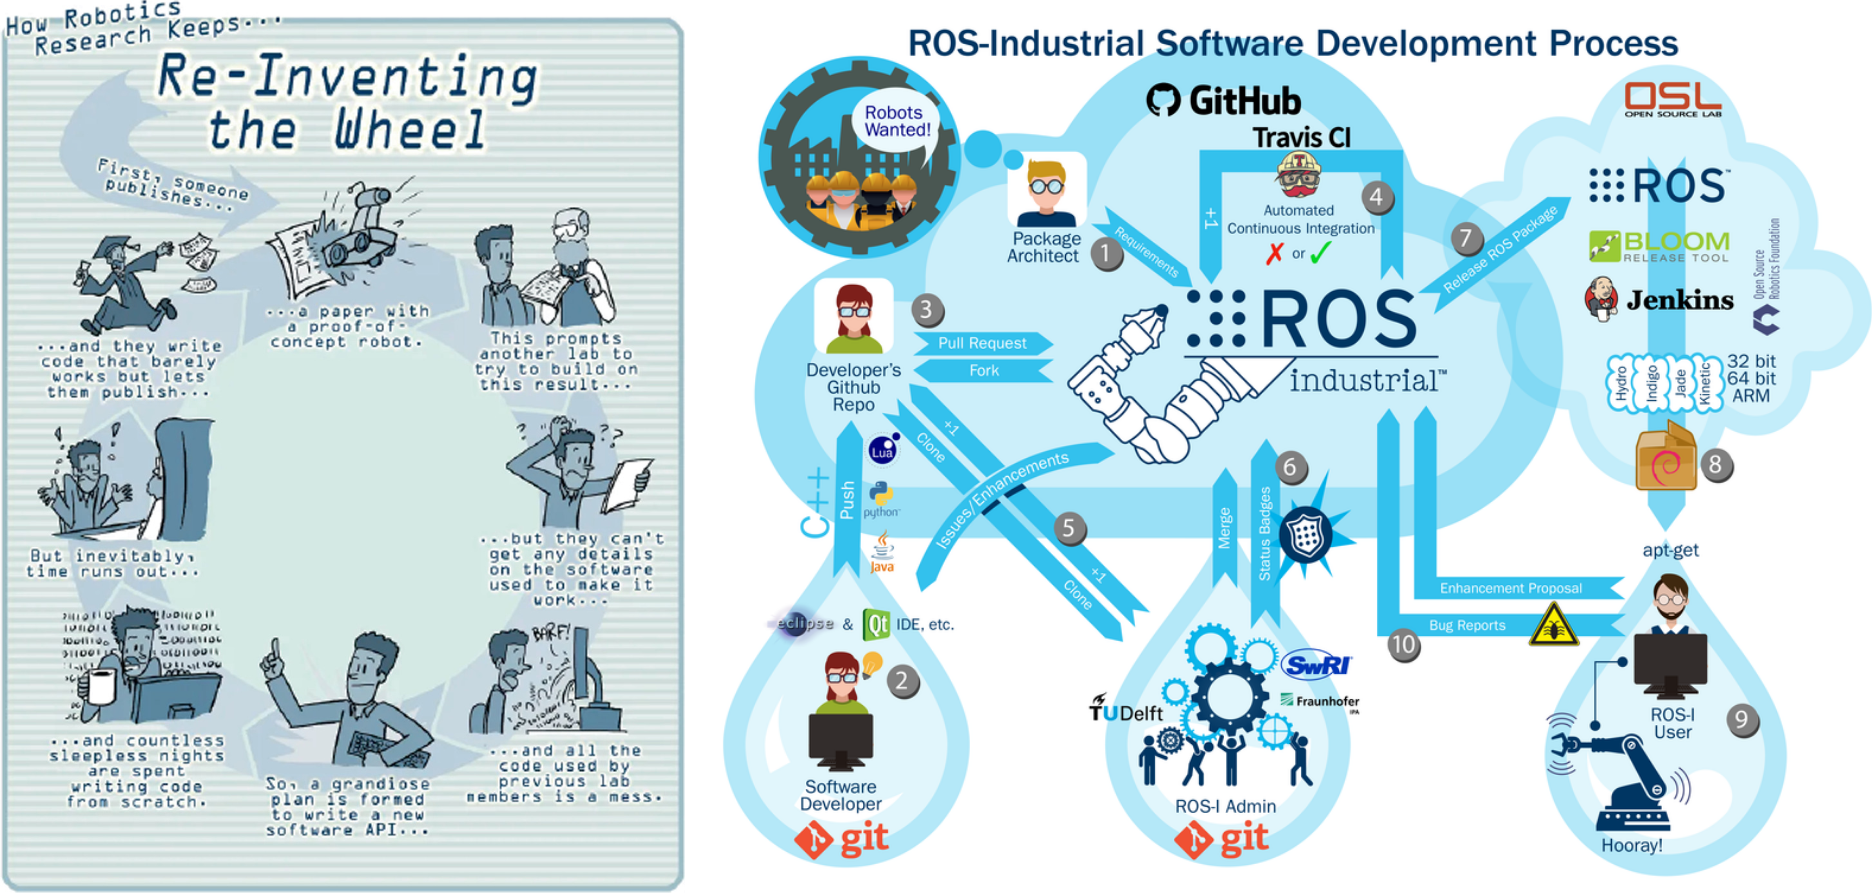
\includegraphics[width=1\textwidth]{ros_problem}
  \end{figure}
\end{frame}

\begin{frame}{Visualización de datos}
  \begin{figure}
    \centering
    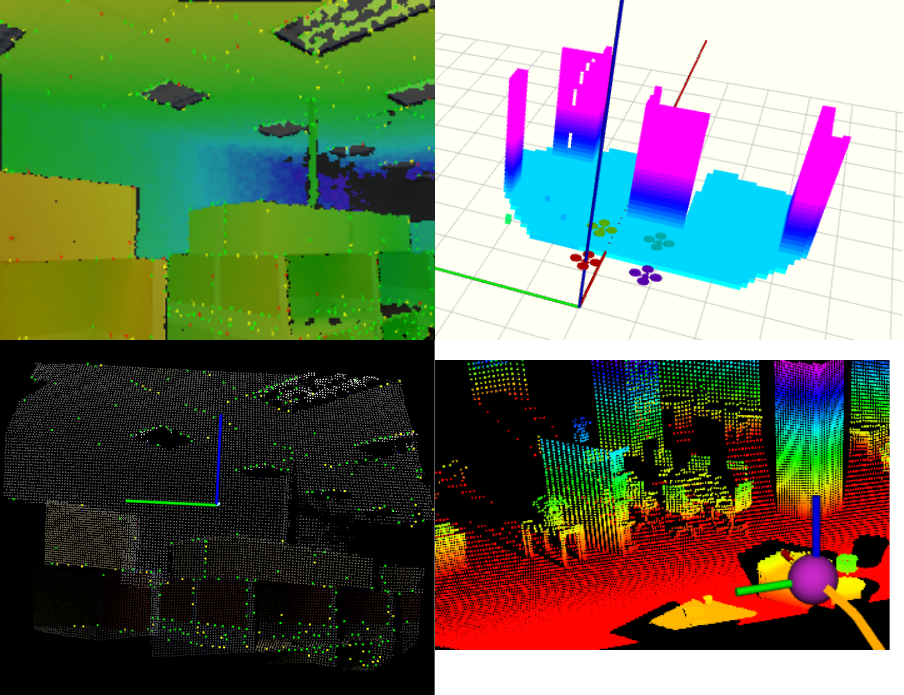
\includegraphics[width=0.6\textwidth]{visual}
  \end{figure}
\end{frame}


\section{Estado del Arte}
\begin{frame}{Estado del Arte}
  \bigskip % Vertical whitespace
  \centering
  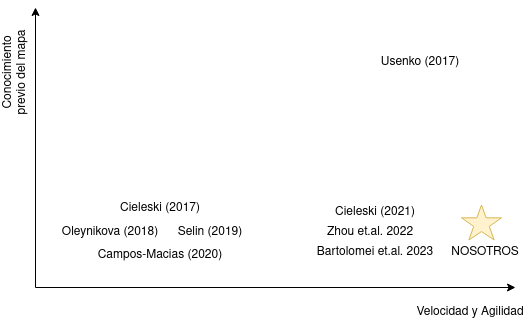
\includegraphics[width=0.6\textwidth]{soa}
  %\begin{tabular}{ | p{4cm} | p{3cm} | p{2.5cm} | p{3.5cm}|}
  %  \hline
  %  \scriptsize REFERENCIA&
  %  \scriptsize REPRESENTACION&
  %  \scriptsize BUSQUEDA&
  %  \scriptsize TRAYECTORIA\\
  %  \hline
  %  \hline
    %--------------------------
  %  \scriptsize \cite{CIESLEWSKI2017}[\citenum{CIESLEWSKI2017}]&
  %  \scriptsize Octomap&
  %  \scriptsize Basado en fronteras&
  %  \scriptsize Control directo de velocidad\\ \hline
    %--------------------------
  %  \scriptsize \cite{USENKO2017}[\citenum{USENKO2017}]&
  %  \scriptsize Cuadr\'{i}cula egoc\'{e}ntrica&
  %  \scriptsize Offline RRT*&
  %  \scriptsize Curvas de Bezier\\ \hline 
    %--------------------------
  %  \scriptsize \cite{MOHTA2017}[\citenum{MOHTA2017}]&
  %  \scriptsize mapa 3D-Local y 2D-Global&
  %  \scriptsize A*&
  %  \scriptsize Programaci\'{o}n cuadr\'{a}tica \\ \hline 
    %--------------------------
  %  \scriptsize \cite{LIN2017}[\citenum{LIN2017}]&
  %  \scriptsize 3D voxel array TSDF&
  %  \scriptsize A*&
  %  \scriptsize Optimizaci\'{o}n cuadr\'{a}tica \\ \hline
    %--------------------------
  %  \scriptsize \cite{PAPACHRISTOS2017}[\citenum{PAPACHRISTOS2017}]&
  %  \scriptsize Octomap&
  %  \scriptsize NBVP&
  %  \scriptsize Control directo de velocidad \\ \hline
    %--------------------------
  %  \scriptsize \cite{OLEYNIKOVA2018}[\citenum{OLEYNIKOVA2018}]&
  %  \scriptsize Voxel Hashing TSDF&
  %  \scriptsize NBVP&
  %  \scriptsize Optimizaci\'{o}n cuadr\'{a}tica \\ \hline
    %--------------------------
  %  \scriptsize \cite{GAO2018}[\citenum{GAO2018}]&
  %  \scriptsize Mapa de cuadr\'{i}cula&
  %  \scriptsize M\'{e}todo de marcha r\'{a}pida&
  %  \scriptsize Optimizaci\'{o}n cuadr\'{a}tica \\ \hline
  %\end{tabular}
\end{frame}

%\begin{frame}
  
%  \centering
%  \begin{tabular}{ | p{4cm} | p{3cm} | p{2.5cm} | p{3.5cm}|}
%    \hline
%    \scriptsize REFERENCIA&
%    \scriptsize REPRESENTACION&
%    \scriptsize BUSQUEDA&
%    \scriptsize TRAYECTORIA\\
%    \hline
%    \hline
    %--------------------------
%    \scriptsize \cite{FLORENCE2018}[\citenum{FLORENCE2018}]&
%    \scriptsize Busqueda basada en visibilidad&
%    \scriptsize 2D A*&
%    \scriptsize Control predictivo por modelo (MPC) \\ \hline
    %--------------------------
%    \scriptsize \cite{SELIN2019}[\citenum{SELIN2019}]&
%    \scriptsize Octomap&
%    \scriptsize Next Best View Planner (NBVP)&
%    \scriptsize Control directo de velocidad \\ \hline
    %--------------------------
%    \scriptsize \cite{BUG2019}[\citenum{BUG2019}]&
%    \scriptsize NA&
%    \scriptsize Swarm Gradient Bug Algorithm (SGBA)&
%    \scriptsize Control directo de velocidad \\ \hline
    %--------------------------
%    \scriptsize \cite{COLLINS2019}[\citenum{COLLINS2019}]&
%    \scriptsize KD Tree $+$ Mapa en Voxel&
%    \scriptsize B\'{u}squeda en Grafo&
%    \scriptsize Movimientos suaves \\ \hline
    %--------------------------
%    \scriptsize \cite{CINVES2021}[\citenum{CINVES2021}]&
%    \scriptsize Octree&
%    \scriptsize Rapidly Exploring Random Trees (RRT)&
%    \scriptsize Basado en contornos \\ \hline
    %--------------------------
%    \scriptsize \cite{RACER2022}[\citenum{RACER2022}]&
%    \scriptsize Octomap HGrid&
%    \scriptsize NBVP&
%    \scriptsize Control directo de velocidad \\ \hline
    %--------------------------
%    \scriptsize \cite{WESTHEIDER2023}[\citenum{WESTHEIDER2023}]&
%    \scriptsize Mapa de cuadrícula&
%    \scriptsize Deep Reinforcement Learning&
%    \scriptsize Control directo de velocidad \\ \hline
    %--------------------------
%    \scriptsize \cite{BARTOLOMEI2023}[\citenum{BARTOLOMEI2023}]&
%    \scriptsize Octomap&
%    \scriptsize Basado en fronteras&
%    \scriptsize Control directo de velocidad \\ \hline
    %--------------------------
%  \end{tabular} 
  
%\begin{figure}
%  \centering
%  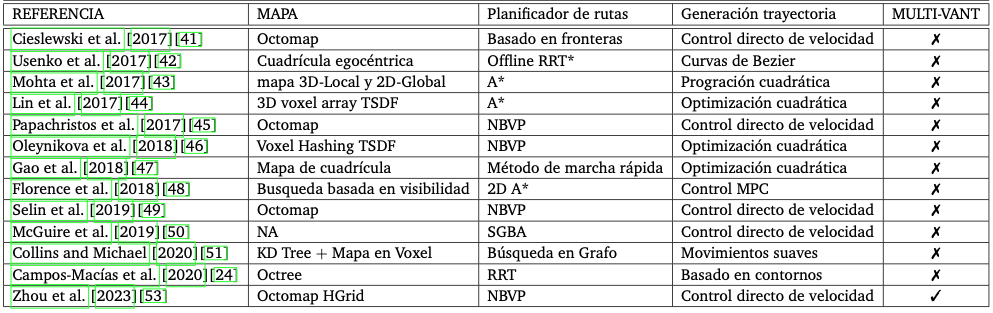
\includegraphics[width=10cm, height=6cm]{estado_del_arte}
%\end{figure}
%\end{frame}

\section{Contribuciones o resultados esperados}
\begin{frame}
  \frametitle{Contribuciones o resultados esperados}
  Se espera que un mecanismo de coordinación en tareas de exploración con múltiples VANTS produzcan mejoras significativas en eficiencia, cobertura y adaptabilidad en la exploración.
  \begin{enumerate}
  \item<1-> Documentación y códigos liberados
    \begin{itemize}
    \item Estrategia coordinada para tareas de exploración multi-VANT.
    \item Arquitectura de software que resuelva los problemas de autonomía para un vehículo aéreo no tripulado.
    \item Protocolo de comunicación multi-VANT que formaran parte de la arquitectura de software
    \end{itemize}
  \item<2-> Validación de la solución en un simulador
    \begin{itemize}
    \item Análisis comparativo de la cobertura alcanzada por la estrategia propuesta.
    %\item Evaluación comparativa del consumo de recursos entre algoritmos de coordinación avanzados y métodos tradicionales.
    \item Evaluación de mecanismos de evasión de obstáculos.
    \end{itemize}
  \item<3-> Tesis impresa
  \end{enumerate}
\end{frame}

\begin{frame}[allowframebreaks,noframenumbering]{Bibliografía}
  \tiny
  \bibliographystyle{abbrvnat}
  \bibliography{test}
\end{frame}

\end{document} 
